\chapter{Software Design} \label{chapter3}
\minitoc
\eject

\section{Introduction}

% We are interested in the evolution of the development of web applications in an economical context.
Computer applications are economically constrained by the cost of both development, and exploitation.
The growth of the web and Software as a Service (SaaS) revealed the importance of these constraints, as the same entity need to carry both development and exploitation in scale of unprecedented size.
% These constraints became even more important, and the costs increased for web applications because with the growth of the web.
% Since the web reached a global scale, these constraints are amplified for applications available on the web.
% These constraints are amplified for web application because the latter are reachable at a larger scale.
In this chapter, we draw a broad view of this duality in software systems projects, to finally refine the scope on our subject of interest, and to define the problematic of this thesis.
% \cit{It is becoming increasingly important to the data-processing industry to be able to produce more programming systems and produce them with fewer errors, at a faster rate, and in a way that modifications can be accomplished easily and quickly.}{W. P. Stevens, G. J. Myers, L. L. Constantine \cite{Stevens1974}}.

% Since the early days of software development as a discipline,
Similarly to many problem solving discipline, in software development the best practices advocate to decompose a problem into many subproblems.
That is to organize the code into independent units, \textit{e.g.} modular programming, structured design \cite{Stevens1974}, hierarchical structure \cite{Dijkstra1968} and object-oriented programming.
% One recurring principle in these approaches is that the units are to be as loosely coupled as possible.
These approaches focus on improving the readability, maintainability and comprehensibility of an implementation.
% We say that they intend to assure the evolution of the software system.
% http://userpage.fu-berlin.de/~ram/pub/pub_jf47ht81Ht/doc_kay_oop_en
% \textit{OOP to me means only messaging, local retention and protection and hiding of state-process, and extreme late-binding of all things. It can be done in Smalltalk and in LISP. There are possibly other systems in which this is possible, but I'm not aware of them.
% Cheers,
% Alan}
These approaches assure the evolution of the implementation of software systems.

The Moore's law \cite{Moore1965} and Dennard's MOSFET scaling \cite{Dennard2007} promised an exponential evolution of the processing power, hence the software industry could always rely on the hardware to increase the execution speed.
But eventually, the clock speed of processors plateaued \ftnt{https://cartesianproduct.wordpress.com/2013/04/15/the-end-of-dennard-scaling/}\cite{Bohr2007}.
The increasing number of transistors predicted by Moore's law needed to be reorganized as several execution units into the same processor.
The hardware could not anymore increase the execution speed without any additional development effort.

The best practices of software development then inherited two goals : to assure the evolution of implementation by decomposing it into subproblems, as well as to decompose the execution onto the several execution units.
As D. L. Parnas showed in 1972 \cite{Parnas1972}, these two decompositions are hardly reconcilable.
It seems impossible to develop a software following a decomposition that satisfies both the evolution, and an efficient parallel execution.

As the economic constraint shifted from development to performance, and with the incentive to leverage the execution power of parallel architectures, intensive work was done to provide tools and model to organize the execution on multiple execution units.
Though, these works often ignore the best practices regarding maintainability.
Increasing performance drastically increases the required development effort.
% For example distributed systems, single instruction multiple data, among others.\nt{TODO not really good examples}

There has been many attempts at reconciling the two goals into a single approach.
But none seems really convincing enough to be widely adopted.
Throughout this chapter, I will classify different works from the community into three categories : focus on implementation evolution in section \ref{chapter3:software-design}, focus on parallel execution in section \ref{chapter3:software-efficiency}, or reconciliation of the two in section \ref{chapter3:reconciliation}.
And finally, I will present the objectives for this thesis in section \ref{chapter3:objectives}.

\section{Software Design} \label{chapter3:software-design}

In order to improve and maintain a software system, one needs the mental representation behind its conception.
Architects, and mechanical engineer draw codified plans to share their mental representations with other architects and building teams.
Similarly software developers write source codes.
But because the source code represents both the plan and its execution, the second aspect tends to shadow the first, and the mental representation is lost in technical the details and optimizations of the implementation.
It then becomes hard or even impossible to quickly grasp without the associated mental representation.
Newcomers, or even the initial author after several weeks, would have difficulties to understand the system.
This problem becomes even more critical as the size of the system grows in size.
Therefore, it is important to decompose the system into smaller subsystem easier to grasp individually.
Such decomposition, improve the readability and comprehensibility hence maintainability of the implementation of a software system.
In this section, we show the theoretical tools for this decomposition, and their application in programming languages.

\subsection{Modularity}

\subsubsection{Structured Programming}

The growing size and complexity of software systems eventually urges the developers to split the problem into isolated subproblems.
To respond to this problem, Dijkstra developed the concept of Structured Programming \cite{Dijkstra1970}.
D. Knuth cited C. Hoare to define Structured Programming as \textit{the systematic use of abstraction to control a mass of details, and also a means of documentation which aids program design} \cite{Knuth1974}.
Dijkstra formalized this procedure on two levels, at a fine grain and at a coarse grain \cite{Dijkstra1968a,Dijkstra1968}.

% A program expressed as a continuous flow of instructions with occasional jumps with 
The \texttt{goto} statement makes the flow of control very hard to follow and understand.
It is called spaghetti code.
Dijkstra advocated instead to decompose the problem into subproblems encapsulated into  structures and reusable functions \cite{Dijkstra1968a}.
It impacts the development at a fine grain.

He also proposed to design complex systems with a hierarchical structure \cite{Dijkstra1968}.
It decomposes a bigger problem at a coarser grain into subproblems encapsulated into layers.
Each layer would abstract a design problem for the upper layers.
This work established grounds for what is know called modular programming.

% Letters to the editor : goto statement considered harmful \cite{Dijkstra1968a}
% The structure of the THE-multiprogramming system \cite{Dijkstra1968}

\subsubsection{Modular Programming}

Modular programming advocates to design a software system as an assembly of modules communicating with each other.
The goal of using modular programming is twofold.
It allows a developer to limit its understanding only to the features isolated inside a module, instead of understanding the whole problem \cite{Stevens1974}.
And it reduces development time by allowing several developers to implement simultaneously different modules \cite{Wong2009,Cataldo2006}.

The criterion to decompose the system into modules are coupling and cohesion \cite{Stevens1974}.
The coupling defines the strength of the interdependence between modules.
It is opposed to cohesion which defines how strongly the features inside a module are related.
Low coupling between modules and high cohesion inside modules imply a better readability and comprehensibility, hence a better maintainability of the implementation of the system.

These two criterion defines how modular is the implementation.
However, it doesn't define how well this organization will stand against the evolution of the implementation.

% (See wikipedia page https://en.wikipedia.org/wiki/Separation_of_concerns)


\subsection{Design Choices}

It is important that the modular organization stand against the evolutions in the specification of the problem, and their consequences in the implementation.
The interfaces between modules, and the contents of these modules need to be well thought.
The information hiding principle, and the separation of concerns are two similar approach to do so.

\subsubsection{Information Hiding Principle}

The information hiding principle helps define the content of modules so as to limit the impact of the evolution to a small portion of the implementation \cite{Parnas1972}.
It advocates to encapsulate a specific design choice in each module to isolate the evolution on this choice from impacting the rest of the implementation.
In this article \cite{Parnas1972}, D. Parnas clearly opposes the organization of modules following the information hiding principle from the one following a pipeline approach to parallelize the execution.
The former organization supports the development evolution, while the latter is more favorable to parallel execution and to performance.
This opposition shows that a program cannot trivially follow an organization that support both development evolution, and performance.

% The structure and value of modularity in software design \cite{Sullivan2001a}
% -> We identify an issue for software designers that neither Parnas’s formulation nor subsequent developments based on it adequately address: A designer is responsible for producing the greatest benefit for any given investment of time, talent, money, and other resources.

\subsubsection{Separation of Concerns}

The Separation of Concern is a design principle advocating that each module is responsible for one and only one specific concern \cite{Tarr1999,Hursch1995}.
For example, the separation of the form and the content in HTML / CSS, or the OSI model for the network stack, are example of separation of concerns.

However, this definition is orthogonal to the original meaning coined by Dijkstra \cite{Dijkstra1982}.
It is interesting to note this difference, as it is related directly to this thesis.
% Initially, it meant the ability to reason independently about different concern about a software system.
The initial definition was about analyzing independently how a system meets different concerns.
Dijkstra gives the example of analyzing independently correctness and efficiency.
It is impossible to encapsulate correctness, or efficiency in a module, they concern the whole system.
In this respect, this thesis is oriented towards separating the concern of development evolution and the concern of performance.
That is to be able to reason on the maintainability of a program, independently than of its performance, and vice versa.
This seems challenging as D. Parnas opposed these two concerns.

In this thesis, we investigate further this opposition to separate the concern of evolution and the concern of performance in the case of a web application.
In the next subsection we investigate the first concern, we present the major programming models used to improve the evolution of an application.

\subsection{Programming Models} \label{chapter3:software-design:programming-models}

Programming languages are designed for developers to follow the best practices mentioned above.
We present two programming models : object oriented programming and functional programming.

\subsubsection{Object Oriented Programming}

% The following list defines Object-Oriented Programming (OOP).
% \begin{enumerate}
% \item Everything is an object.
% \item Communication is performed by objects communicating with each other, requesting that objects perform actions. Objects communicate by sending and receiving messages. A message is a request for action, bundled with whatever objects may be necessary to complete the task.
% \item Objects have their own memory, which consists of other objects.
% \item Every object is an instance of a class. A class simply represents a grouping of similar objects, such as integers or lists.
% \item The class is the repository for behavior associated with an object. That is, all objects that are instances of the same class can perform the same actions.
% \end{enumerate}

Alan Kay, who coined the term, states that Object Oriented Programming (OOP) is about message-passing, encapsulation and late binding.
(There is no scholar reference for that, only a public mail exchange\ftnt{http://userpage.fu-berlin.de/~ram/pub/pub\_jf47ht81Ht/doc\_kay\_oop\_en}.)
This original definition is strongly related to modular programming.
It helps encapsulate both the data, and the functions to process this data in an isolated, loosely coupled module.
The very first OOP language was Smalltalk \cite{Goldberg1984}.
It defined the core concept of OOP, and is inspired by LISP and by the definition of the Actor Model, which we will define in the next section.

% Illustration of multiple cells, as Alan Kay thought of biology when developing the object-oriented concepts.
% http://userpage.fu-berlin.de/~ram/pub/pub_jf47ht81Ht/doc_kay_oop_en
% I thought of objects being like biological cells [...] able to communicate with messages ...

Object-Oriented Programming evolved to adopt as well the concepts of class, inheritance and polymorphism.
The major languages of the software industry feature this Object-Oriented approach.
We can cite C++ and Java as the emblematic figures of OOP.

Though, the field test seems to have had reason of this strict version of OOP.
The trends in programming language seems to digress from the pure Object-Oriented approach to evolve toward an approach closer to Functional Programming.
Indeed Javascript, Ruby and Python adopt functional features such as dynamic typing and higher-order functions.

% \paragraph{Object Calisthenics}

% Object calisthenics are defined as the chapter 6 of \textit{The Thoughtworks Anthology} \cite{Bay2008}.
% It is an exercise for developers presented as a list of 9 rules to follow to enforce maintainability and readability on source code \ftnt{http://www.cs.helsinki.fi/u/luontola/tdd-2009/ext/ObjectCalisthenics.pdf}.

% Some of these rules are direct implementations of the more general concept of separation of concerns, and information hiding.
% As an example, rule 7 \textit{Keep all entities small} advocate that entities should have a concise concern.
% Other rules are just syntactic guides to improve readability and comprehensibility.


% See Object calisthenics 
% - http://williamdurand.fr/2013/06/03/object-calisthenics/
% - http://www.cs.helsinki.fi/u/luontola/tdd-2009/ext/ObjectCalisthenics.pdf



\subsubsection{Functional Programming} \label{chapter3:software-design:programming-models:functional-programming}

% \cit{All problems in computer science can be solved by another level of indirection}{Butler Lampson}

Functional programming is often associated to its purest form, manipulating only expressions - in place of operation statements - and forbidding state mutability.
However, the essence of functional programming is not as strict, it resides in higher-order functions and lazy evaluation.
Two features that major programming languages now commonly adopt.

\paragraph{Higher-Order Function}

Languages providing higher-order functions allows to manipulate functions like any other primary value : to store them in variables, or to pass them as arguments.
Higher-order functions replace the needs for most modern object oriented programming design patterns \ftnt{http://stackoverflow.com/a/5797892/933670}.
Higher-order functions and lazy evaluation help loosen the couple between modules, and improve their re-usability.
\textit{In fine}, it helps developers to write applications that are more maintainable, and upgradeable \cite{Hughes1989}.

\paragraph{Closures}

Most languages use closures to implement lexical scope with higher-order functions \cite{Sussman1998}.
A closure is the association of a function and the data context from its creation.
It allows this function to access variable from this context, even when invoked outside their scope, for example when passed as an argument to another module.

It loosen the couple between modules, and helps define more generic and reusable modules.
However, it increase their dependencies during the execution.
Indeed, by exchanging closures, two modules intricately share their contexts of execution.

\paragraph{}

Functional programming greatly improves the resilience of implementation to the evolution of their specification.
However, it requires a global memory to share the context of execution among modules.
As we will see in the next section, sharing memory makes parallelism difficult.
In this regard, the concern of evolution and the concern of performance seem incompatible.


\endinput

\subsubsection{Modularity based on Design Decisions}

Designing Software for ease of extension and contraction \cite{Parnas1979}

Design Rules: The Power of Modularity Volume 1 \cite{Baldwin1999}
A reference book, but I can't get it.
\section{Efficiency Focused Platforms} \label{chapter3:software-efficiency}

Both the academia and the industry proposed solutions with efficiency in mind to cope with the limitations the previous section concludes on.
Section \ref{chapter3:software-efficiency:concurrency} presents the concurrent and parallel programming paradigms, and their programming models. % oriented on performance rather than productivity.
Section \ref{chapter3:software-efficiency:adoption} presents the adoption steered by the efficiency of parallel programming.
Section \ref{chapter3:software-efficiency:productivity-limitations} presents the consequences of parallelism on productivity.
Finally, section \ref{chapter3:software-efficiency:summary} summarizes the three previous sections in a table.

\subsection{Concurrency} \label{chapter3:software-efficiency:concurrency}

\begin{figure}[!h]
\begin{center}
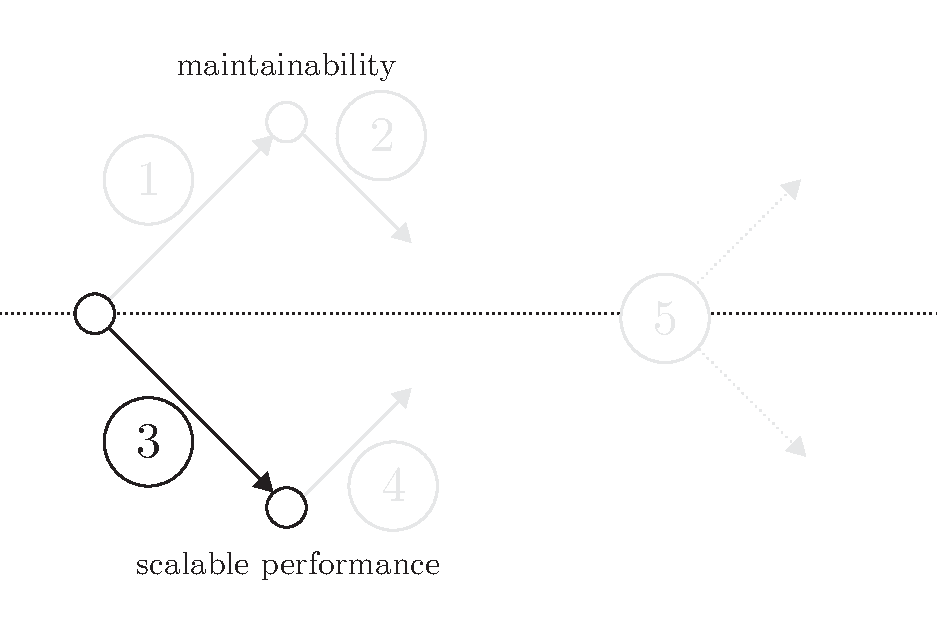
\includegraphics[width=0.6\textwidth]{../ressources/state-of-the-art-3.pdf}
\end{center}
\caption{Focus on Efficiency}
\label{fig:state-of-the-art-3}
\end{figure}

Web servers need to be able to process huge amount of concurrent operations in a scalable fashion.
Concurrency is the ability to make progress on several operations roughly simultaneously.
It implies to draw memory boundaries to define independent regions, or to define causality in the execution of tasks.
When both boundaries and causality are clearly defined, the tasks are independent and can be scheduled in parallel to make progress strictly simultaneously.

The definition of independent tasks allows the fine level synchronization within a task, and coarse level message passing between the tasks required for performance efficiency.
The synchronization of execution at a fine level assures the invariance on the shared state, and avoid communication overhead.
The message-passing at a coarser level assures the parallelism.
The two are indispensable for efficiency.

\subsubsection{Concurrent Programming} \label{chapter3:software-efficiency:concurrency:concurrent-programming}

% \cit{Building concurrent programming is like building a steam engine through a keyhole}{TODO}

\illustration{feu rouge et rond point}
Concurrent programming provides the mechanisms to assure atomicity of concurrent operations.
They define the causal scheduling of execution and assure the invariance of the global memory.
There are two scheduling strategies to execute concurrent tasks on a single processing unit, cooperative scheduling and preemptive scheduling.

\begin{description}
\item[Cooperative Scheduling] allows a concurrent execution to run until it yields back to the scheduler.
Each concurrent execution has an atomic, exclusive access on the memory.
\item[Preemptive Scheduling] allows a limited time of execution for each concurrent execution, before preempting it.
It assures fairness between the tasks, such as in a multi-tasking operating system.
But the unexpected preemption breaks atomicity, the developer needs to lock the shared state to assure atomicity and exclusivity.
\end{description}

The next paragraphs presents the programming model for these scheduling strategy, the event-driven programing model based on cooperative scheduling, and the multi-threading programming model based on preemptive scheduling.
Additionally, they present two alternatives to these two main programming models, lock-free data-structures and Fibers.

\paragraph{Event-Driven Programming}

Event-driven execution model queues concurrent tasks needing access to shared resources.
The tasks are explicitely defined by the developer.
The concurrent tasks are schedule sequentially to assure exclusivity, and cooperatively to assure atomicity.
% Web servers needs to be highly concurrent, and efficient.
It is very efficient for highly concurrent applications, as it avoids contention due to waiting for shared resources like disks, or network.
Several execution model rely on this execution model, like \ImplementationsOf{Event-driven programming}.
As well as some web servers like Flash \cite{Pai1999}, Ninja \cite{Gribble2001} thttpd\ftnt{http://acme.com/software/thttpd/} and Nginx\ftnt{https://www.nginx.com/}.

% However, a drawback of this model was that the execution context is lost at each event.
% The developer needs to explicitly transfer the relevant state to continue the execution from one event execution to another.

% + Fibers \cite{Adya2002}
% + Capricio \cite{Behren2003a} - User cooperative threads (also known as fibers / green threads)

% The problem of losing the execution context disappears with closures in higher-order programming.
% \nt{link with the previous paragraph}
% Moreover, the continuation passing style used in higher-order programming requires the developer to be aware of the asynchronous rupture in the execution, so as to assure atomicity \cite{Sussman1998}.
% And because an asynchronous call doesn't wait for the completion of the operation, the asynchronous control flow is not limited to be linear like in threads. \nt{more about that}
% Multiple asynchronous calls are made in parallel.

% + TAME \cite{Krohn2007} - event-based solution without stack ripping in C (it is like closure, but for C)
% + Node.js - \ftnt{https://nodejs.org/en/}
% + Vert.X - \ftnt{http://vertx.io/} node like + thread / worker capabilities

But the event-driven model is limited in performance.
The concurrent tasks share the same memory, and cannot be scheduled in parallel.
The next paragraph presents work intending to improve performance by reducing the atomic portions of operations to a minimum. % by reducing the sequential portions to a minimum to increase the possibilities of parallelism.

\paragraph{Lock-Free Data-Structures}

The wait-free and lock-free data-structures use atomic operations small enough so that locking is unnecessary \cite{Lamport1977,Herlihy1988,Herlihy1990,Herlihy1991,Anderson1990}.
They are based on instructions provided by transactional memories \cite{Harris2010} that combine read and write instructions,
They provide concurrent implementations of basic data-structures such as \ImplementationsOf{Lock-free Data-Structures}.

However these atomic operations are scheduled sequentially, which limits parallelism.
The next paragraphs present multi-threading, which, contrary to the event-driven model, requires the developer to explicitly define atomicity.
% using coarser granularity of atomic execution and exclusivity.

% Reference papers :
% Concurrent reading and writing \cite{Lamport1977}
% Impossibility and universality results for wait-free synchronization \cite{Herlihy1988}
% A methodology for implementing highly concurrent data structures \cite{Herlihy1990}
% Wait-free synchronization \cite{Herlihy1991}

% Book :
% The virtue of Patience: Concurrent Programming With And Without Waiting \cite{Anderson1990}

\paragraph{Multi-Threading Programming}

Threads are the small execution containers sharing the same memory execution context within an isolated tasks \cite{Dijkstra1968}, and scheduled in parallel with fork/join instructions \cite{Randall1998,Frigo1998,Leiserson2010}.
They execute statements sequentially waiting for completion, and are scheduled preemptively to avoid blocking the global progression.
The preemption breaks the atomicity of the execution, and the parallel execution breaks the exclusivity of memory accesses.
To restore atomicity and exclusivity, hence assure the invariance, multi-threading programming models provide synchronization mechanisms, such as \ImplementationsOf{Multi-threading programming}.

Developers tend to use the global memory extensively, and threads require to protect each and every shared memory cell.
This heavy need for synchronization leads to bad performances, and is difficult to develop with \cite{Adya2002}.

\paragraph{Cooperative Threads}

Cooperative threads, or fibers join the advantage of sequential waiting, with the advantage of cooperative scheduling \cite{Adya2002,Behren2003a}.
It avoids splitting the execution into atomic tasks nor use synchronization mechanisms to assure exclusivity.
A fiber yields the execution to another fiber to avoid blocking the execution during a long-waiting operation, and recovers it at the same point when the operation finishes.
However, developers need to be aware of these yielding operation to preserve the atomicity\ftnt{https://glyph.twistedmatrix.com/2014/02/unyielding.html}.

\paragraph{Limitation of Concurrent Programming}



% Moore's law \cite{Moore1965} which forecasts the density of transistors per processing unit, was wrongly interpreted to promise the exponential evolution in the sequential performance of the processing unit, and the assurance for the software industry of always faster hardware.
% But as transistors attained a critical size, the reduction in power required by transistor predicted by the Dennard's MOSFET scaling \cite{Dennard2007} stopped\ftnt{https://cartesianproduct.wordpress.com/2013/04/15/the-end-of-dennard-scaling/}.

Concurrent programming provides the synchronization required to assure sequentiality of execution within a task and the causal ordering between tasks.
However, multi-threading imposes sequentiality between tasks as well.
This global sequentiality is excessive ; it impacts performance, and is difficult to manage efficiently.

The causal ordering between tasks proposed by the event-driven execution model is sufficient to assure correctness of execution \cite{Lamport1978,Reed2012}.
But because of the lack of memory isolation, the concurrent tasks are not scheduled in parallel.

Parallel programming is the only solution for efficiency, at the expense of development efforts to explicitely define the memory isolation of concurrent tasks and their communications by message pasing.

% Synchronization mechanisms define shared memory, and lock-free data structures improve the parallel portion of execution, but the performance remains limited.

\paragraph{}

The table \ref{tab:efficiency-concurrency} presents a summary of the analysis of performance of the platforms presented in this section.

\ConcurrentEfficiencyTable{tab:efficiency-concurrency}



% Concurrent programming is a compromise to process operations simultaneously, by introduction synchronization to assure the exclusion required for shared states.


% The ever growing number of transistor predicted by Moore's law \cite{Moore1965} are arranged in parallel architecture to continue increasing the performance of processing units.
% Parallel programming became the only solution for efficiency, at the expense of development effort.


% This section presents the parallel programming solutions and their limitations in accessibility, and then the improvements to overcome these limitations.


% \nt{The shared-nothing architecture \cite{Stonebraker1986}}


\subsubsection{Parallel Programming} \label{chapter3:software-efficiency:concurrency:parallel-programming}


Concurrent programming allows to define the tasks scheduling causally.
% The ordering of operations is local within a synchronous execution, while the concurrent executions are causally ordered.
% It leads to parallel execution with some coordinations such as synchronization, immutability or isolation.
Concurrent tasks can be scheduled in parallel only if their memory are isolated.

The Flynn's taxonomy \cite{Flynn1972} categorizes parallel executions in function of the multiplicity of their flow of instruction and data.
Parallel programming models belong to the category Multiple Instruction Multiple Data (MIMD), which is further divided into Single Program Multiple Data (SPMD) \cite{Auguin1983,Darema1988,Darema2001} and Multiple Program Multiple Data (MPMD) \cite{Chang1997,Chan2004}.
SPMD defines a single program replicated on many processing units \cite{Culler,Johnson1995,K.ManiChandy2005} -- it is derived from the multi-threading programming model presented in section \ref{chapter3:software-productivity:concurrency:concurrent-programming}.
While MPMD defines multiple parallel tasks in the implementation \cite{Grimshaw1991,Foster1995b,Foster1996}.

\nt{schema of SPMD and MPMD}

% , communicating by message passing \cite{Sunderam1994,Snir1996,Walker1996}, SOAP, or the more recent REST protocols.

This section presents MPMD platforms allowing to define isolated tasks.
It presents theoretical and programming models on asynchronous communication and isolated execution for parallel programming.
It then presents stream processing programming models.
And finally, it concludes on the limitations of parallel programming regarding productivity. 



% % \paragraph{Asynchronous and Isolated Process Parallelism}

% The Flynn's taxonomy \cite{Flynn1972} is commonly used to categorize parallel executions.
% It separates the flow of instructions, and the flow of data, each being single or multiple.
% All the current parallel programming models belong to the category Multiple Instruction Multiple Data (MIMD), which is further divided into Single Program Multiple Data (SPMD) \cite{Auguin1983,Darema1988,Darema2001} and Multiple Program Multiple Data (MPMD) \cite{Chang1997,Chan2004}.
% % The difference between SPMD and MPMD holds on the distinction of instruction pool between the threads of execution.
% % SPMD implies to replicate the same program on all the processing units, while MPMD implies to define different programs for every processing units.

% \begin{figure}
% \begin{center}
% 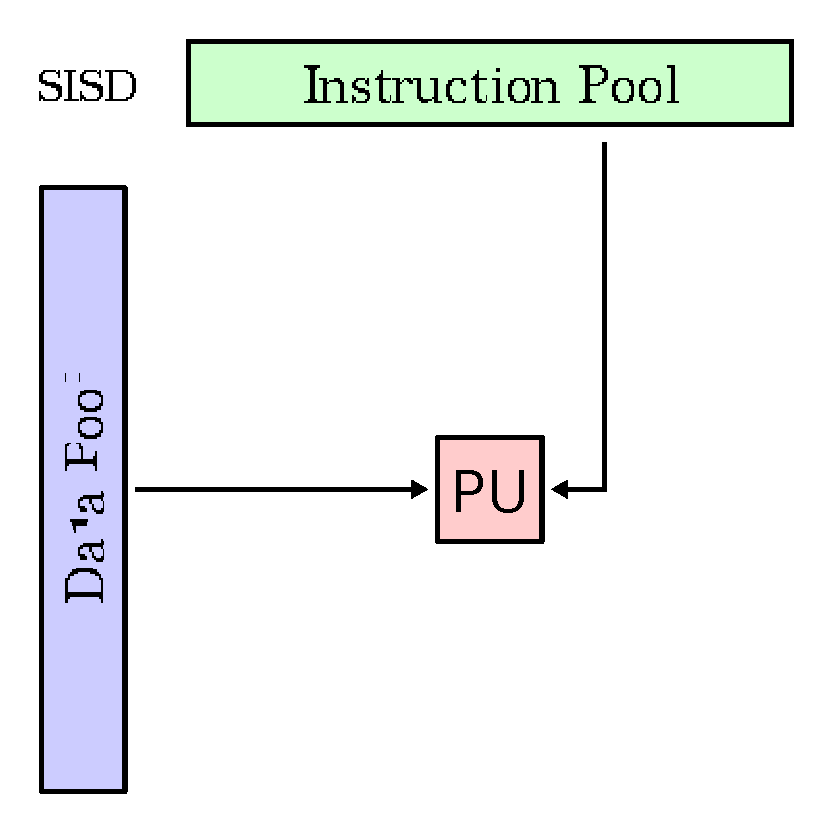
\includegraphics[width=0.2\textwidth]{../ressources/SISD.pdf}
% 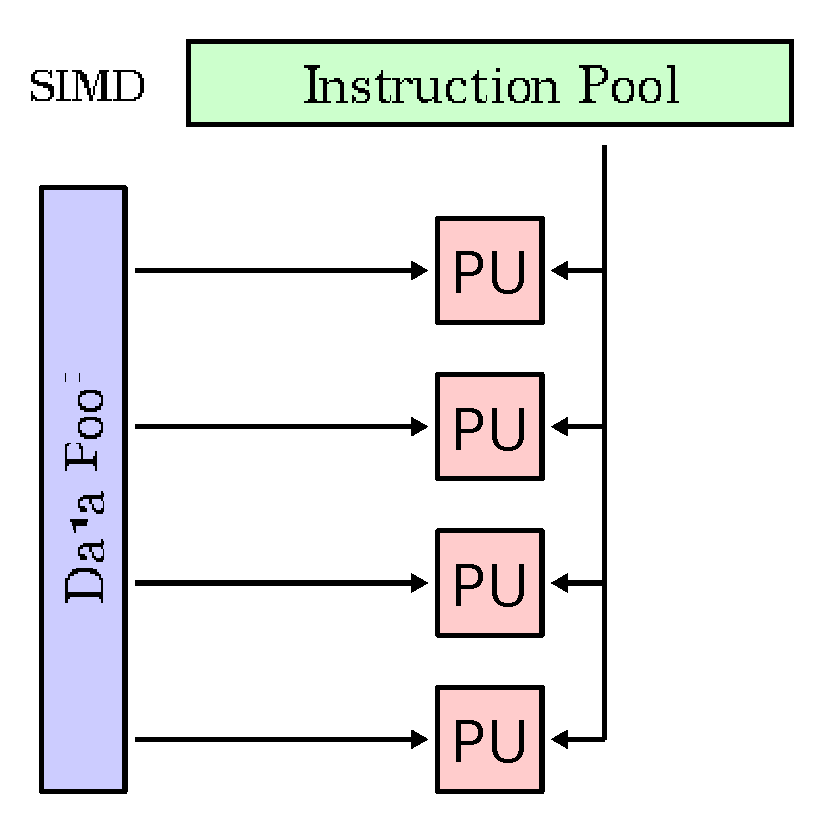
\includegraphics[width=0.2\textwidth]{../ressources/SIMD.pdf}
% 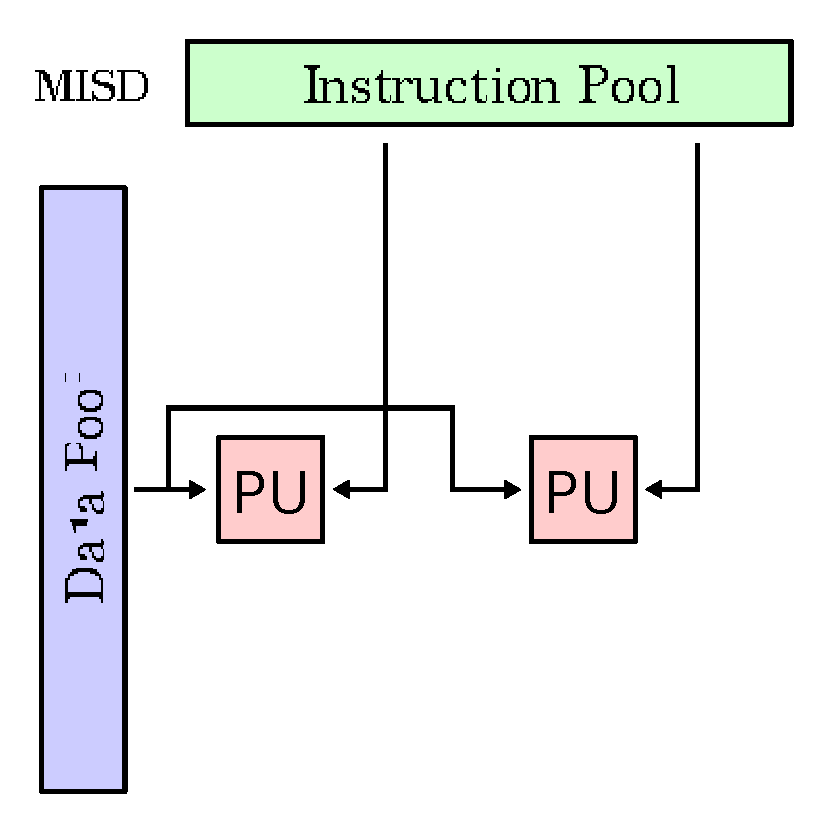
\includegraphics[width=0.2\textwidth]{../ressources/MISD.pdf}
% 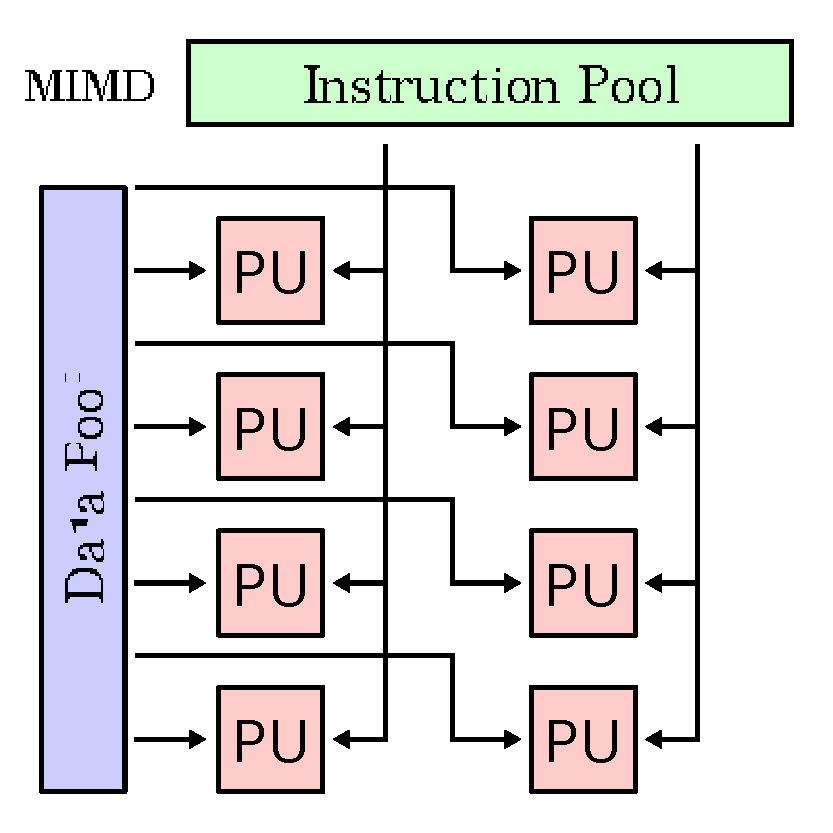
\includegraphics[width=0.2\textwidth]{../ressources/MIMD.pdf}\\
% by I, Cburnett. Licensed under CC BY-SA 3.0 via Commons
% \url{https://commons.wikimedia.org/wiki/File:{SISD,SIMD,MISD,MIMD}.svg}
% \end{center}
% \caption{Flynn's taxonomy of parallelism}
% \label{fig:flynn-taxonomy}
% \end{figure}


% % The difference between SPMD and MPMD is in the representation of the execution in implementation.
% SPMD defines a single program replicated on many processing units.
% Examples of SPMD programming languages are
% Split-C \cite{Culler},
% CRL \cite{Johnson1995} and
% Composite C++ \cite{K.ManiChandy2005}.
% %
% MPMD defines multiple processes in the implementation, communicating by message passing, using PVM \cite{Sunderam1994}, MPI \cite{Snir1996,Walker1996}, SOAP, or the more recent REST protocols.
% Examples of MPMD programming languages are
% Mentat \cite{Grimshaw1991},
% Fortran M \cite{Foster1995b} and
% Nexus \cite{Foster1996}.

% SPMD is close to the model presenting parallel improvements over modular programming presented in section \ref{chapter3:software-productivity:programming-models}.
% While MPMD is closer to the programming models based on isolated process presented in the remaining of this section.
% The coordinations between these processes is done by message passing, using PVM \cite{Sunderam1994}, MPI \cite{Snir1996,Walker1996}, SOAP, or the more recent REST protocols.

\paragraph{Theoretical Models}

The event-driven programming model used to cope with asynchronous communications allows the causal scheduling of concurrent tasks.
% The total ordering of execution imposed by sequential execution is excessive.
This causal scheduling is sufficient to assure correctness in a distributed system \cite{Lamport1978,Reed2012}.
% As Lamport showed \cite{Lamport1978}, and Reed related later \cite{Reed2012}, causal order is sufficient to execute correctly a system in parallel, such as a distributed system.
% The total ordering of execution provided by synchronization is an overkill.
The Actor model allows to express the causal ordering of computation as a set of parallel actors communicating by asynchronous messages \cite{Hewitt1973a, Hewitt1977, Clinger1981}.
In reaction to a received message, an actor can create other actors, send messages, and choose how to respond to the next message.
% All actors are executed concurrently, and communicate asynchronously.
% An asynchronous communication implies that the sender continues its execution immediately after sending the message, before receiving the result of the initiated communication.
Additionally, the communication in reality are too slow compared to execution to be synchronous, and are subject to various faults and attacks \cite{Lamport1982}.
The Actor model takes these physical limitations in account \cite{Hewitt1977a}.

% In the Actor Model, everything is an actor, even the simplest types like numbers.
% This level of granularity is unachievable in practice due to overhead from the asynchronous communications.
% Most implementations adopt a granularity on the process or function level.

Similarly, coroutines are autonomous programs which communicate with adjacent modules as if they were input and output subroutines \cite{Conway1963}.
It defines a pipeline to implement multi-pass algorithms.
Similar works include the Communicating Sequential Processes (CSP) \cite{Hoare1978, Brookes1984}, and the Kahn Networks \cite{Kahn1974, Kahn1976}.

\subsubsection{Summary of Concurrent and Parallel Programming Models}

Table \ref{tab:efficiency-parallel} presents a summary of the analysis of the paradigm presented in the previous paragraphs.

\ParallelEfficiencyTable{tab:efficiency-parallel}







\subsection{Adoption} \label{chapter3:software-efficiency:adoption}

\begin{figure}[!h]
\begin{center}
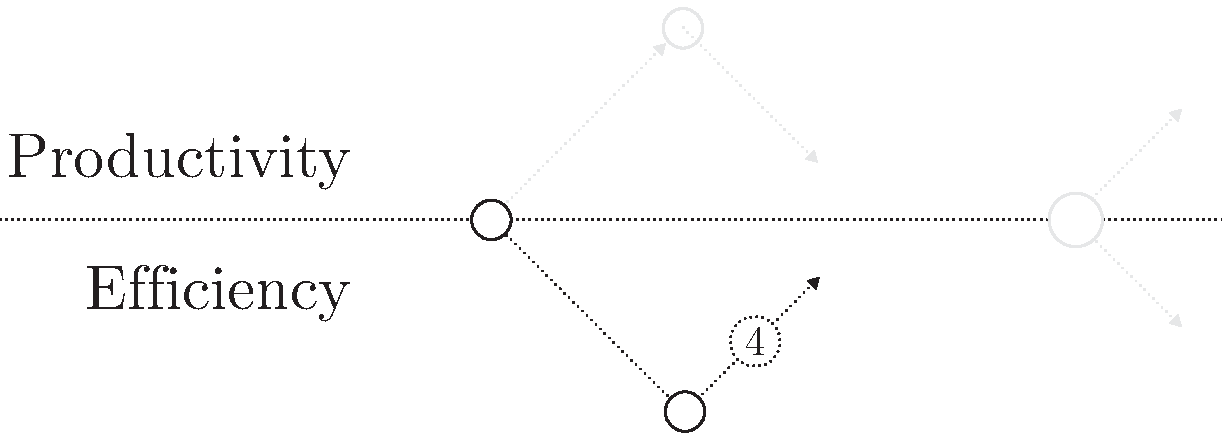
\includegraphics[width=0.6\textwidth]{../ressources/state-of-the-art-4.pdf}
\end{center}
\caption{Steering back toward Productivity}
\label{fig:state-of-the-art-4}
\end{figure}


\illustration{mars rover}
When the need for efficiency is higher than the need for productivity, the adoption is steered by the industry more than the community.
If the industry really needs a platform, it will commit the required development effort despite a low productivity.
% If there is industrial need, there will be maintenance.
The platforms for the Mars Rover or the banking systems are 30 years old, yet the industry continues to maintain them.
%, and there is no community to maintain it.
The platform presented in this section emerged from the academia and the industry but are often barely known by the larger community of developers.
The more the platform abandons productivity, the less it will be supported by the community.

% The performance improvements comes directly from the industry requirements.

% All these system make sense in industrial context.
% Industries have the money to fund the necessary research.

% However, the context of this thesis is different from a classical industrial context.
% During the bootstrap of a web application project, the economical context requires technologies with strong community, to pick talents from to grow the team quickly and effortlessly.
% It also requires these technologies to be of industrial standard, to build a reliable product.
% And these technology must be compatible with web technologies.
% \begin{itemize}
% \item Community support
% \item Industrial need
% \end{itemize}


% \nt{review this paragraph and the transition to the next section}
% The field of concurrent programming is so vast it is impossible to relate here every programming languages.
% The previous examples are only the best known.
% The next focus focuses on streaming real-time applications.

% \comment{transition on lazy evaluation equivalence to stream. lazy evaluation + side effects + concurrency = streams}



% + all the solutions that have a great industrial impact (storm, millwheel and co)



% \subsubsection{Exection Decomposition}


% The programming paradigms presented above are implemented in many existing programming languages.
% All major programming languages implements some form of concurrency or parallelism mechanism.
% The next paragraphs presents these implementations by the industry and the community.
% And more specifically, how they deal with the need to decompose the execution.

% \paragraph{Event-Loop}

% The event-loop model, featured by the DOM and Node.js with Javascript, allows concurrency but not parallelism.
% It decomposes the execution into sequences of callbacks functions, but keep the memory shared.

% As presented in the previous section, Javascript is currently one of the most used language.
% This asynchronous programming model without the memory decomposition seems to be easy to develop with.
% It is used extensively in the community as well as in the industry.
% However, when the programming model requires the memory to be decompose, in order to get parallelism, it becomes more complicated to develop with, as presented in the next paragraphs.

% \paragraph{Multi-Threading}

% The multi-threading model allows concurrency and parallelism on certain execution region.
% It decomposes the execution into fork-join threads, and the memory is shared, but protected with locks.
% The protection of the shared memory is the reason concurrent programming is difficult to manage for most developers.
% Multi-threading is difficult to program with, and for this reason, it leads to poor performances.
% It is not heavily used in the community, where the need for concurrency is limited.
% In the industry, where the concurrency is often required, multi-threading is abandoned for other paradigms, such as the event loop or the actor model.

% \paragraph{}

% The event-loop requires an execution decomposition, but not a memory decomposition.
% This paradigm is heavily adopted by both the community and the industry.
% On the other hand, the multi-threading paradigms with locks requires an execution decomposition, and light memory decomposition.
% This paradigms is not heavily used in the community, and is being abandoned by the industry.
% This comparison between the event-loop and the multi-threading paradigms seems to indicate that the memory decomposition heavily restrains the adoption by the community.
% Hence, it impacts the productivity required for the adoption in the economical context of this thesis, as shown in table \ref{scalability-execution-decomposition}.

\subsubsection{Concurrent Programming}

Most programming languages implementation supports concurrent programming somehow.
Either with multi-threading or event-driven programming.
These two are highly adopted by both the industry and the community, as presented in section \ref{chapter3:software-productivity:adoption}.

On the other hand, lock-free data structures and cooperative threads comes from the academia, similarly to functionnal programming, and did not encounter significant adoption from the community.

Table \ref{tab:adoption-concurrent} presents a summary of the adoption of concurrent programming models.

\ConcurrentAdoptionTable{tab:adoption-concurrent}

\subsubsection{Parallel Programming}

There exists several platforms directly inspired by the actors model, like \ImplementationsOf{Actor Model}.
Scala is a programming language unifying the object model and functional programming.
Akka is a framework based on Scala, following the actor model to build highly scalable and resilient applications.
Play is a web framework based on top of Akka.
And Erlang is a functional language designed by Ericsson to operate networks of telecommunication devices \cite{Armstrong1993,Nelson2004,Armstrong2014}
% Nelson2004 is not very good, find another better citation.

There are as well other platforms inspired by other theoretical model, like \ImplementationsOf{Concurrent Sequential Processes}, inspired by Coroutines and CSP.
Go is an open source language initiated by Google to build highly concurrent services.

These examples of implementation are largely used in the industry, but are almost unknown outside of it.
They are backed by strong, but small passionated communities.

However, the organization in independent tasks is hardly compatible with the modular organization presented in the previous section.
It is difficult for developers to manage the superposition of these two organizations, tasks and modules.
This superposition makes these platforms accessible only to an elite in the industry supporting it.
The next paragraphs present platforms mitigating the difficulty stemming from the duality between execution decomposition and modularity.

\paragraph{Tasks Organization and Communications}

To reduce the difficulties of the superposition of tasks and modules, algorithmic skeletons propose predefined patterns of organization to fit certain types of problems \cite{Cole1988, Dean2008, McCool2010, Gonzalez-Velez2010}.
Developers specialize a skeleton and focus on their problem independently of the required communication.
These solutions are hardly used by the community, but are crucial in some industrial contexts.
A famous example is the map/reduce pattern introduced by Google \cite{Dean2008}.

% \nt{Link with DSMS}
% As there is similtudes between SQL-like languages, functional structures, and algorithmic skeletons, the latter can be seen as a tentative to merge the more descriptional features of the former into imperative programming.
% Indeed, among the Algorithmic skeletons, we can cite Map / reduce, which are functional structures, but are somehow equivalent to the select and aggregate functions of SQL.
% The pipeline architecture for data stream processing presented in section \ref{chapter3:software-efficiency:dataflow-pipeline} can be considered as algorithmic skeletons.

% However, they introduce limitations and difficulties, as the developer must fit its problem into the skeletons.
% One of this difficulties, it that a common memory is impossible to use.
% Developers needs to think in terms of message passing instead of a global memory, which, as we saw in previous section, is incompatible with best practices.

% Introducing 'Bones': a parallelizing source-to-source compiler based on algorithmic skeletons \cite{Nugteren2012}

\paragraph{Tasks Granularity}

The Service Oriented Architectures (SOA) allows developers to express an application as an assembly of services connected to each others.
Some examples of SOA platforms are \ImplementationsOf{Service Oriented Architecture}.
It allows to adjust the granularity of tasks to help developers to better fit the tasks organization with the modular organization \cite{Adam2008}.

More recently, Microservices are tackling the same challenge on the web \cite{Fernandez-Villamor2010,Fowler2014,Namiot2014}.
Some examples of Microservices are \ImplementationsOf{Microservices}.
They are very recent, and it is difficult to asses their usage in the community nor the industry.
But they seems to be increasingly adopted, both in the industry and in the community.

% In modular programming a module protects the rest of the implementation from the consequences of the design choice its encapsulate, while a service encapsulate a specific task, with possible consequences on the adjacent services.

% In a fine enough granularity of service, each service becomes so simple, it can limits the consequences of its modification.

\paragraph{}

The parallel programming platforms previously presented allow to build generic distributed systems.
In the context of the web, a real-time application must process high volumes streams of requests within a certain time.
The next paragraphs present platforms focusing on this challenge.
% Because these systems are key to business, their reliability and latency are of critical importance.
% The next paragraphs present the platform meeting these requirements required for industry adoption.
% Again, these platforms emerged from the academia and the industry and did not always gather huge community enthusiasm.


\subsubsection{Stream Processing Systems}

% Otherwise, input data may be lost or output data may lose their value.
% These requirements are challenging to meet in the design of such system.

\paragraph{Data-stream Management Systems}

Database Management Systems (DBMS) historically processed large volume of data, and they naturally evolved into Data-stream Management System (DSMS) to processed data streams as well.
Because of this evolution, they are in rupture with MPMD platforms presented until now.
They borrows the syntax from SQL to run requests in parallel on continuous data streams.
The computation of these requests spread over a distributed architecture.
% Among the early works, we can cite
% NiagaraCQ \cite{Chen2000,Naughton2001},
% Aurora \cite{Abadi2003,Abadi2003a,Balakrishnan2004} which evolved into
% Borealis \cite{Abadi2005},
% AQuery \cite{Lerner2003},
% STREAM \cite{Arasu2003,Arasu2005} and
% TelegraphCQ \cite{Krishnamurthy2003,Chandrasekaran2003}.
% More recently, we can cite
Some recent examples are \ImplementationsOf{Data Stream System Management}.


\paragraph{Pipeline Architecture}

% As presented in the previous section, streaming composition allows a loosely coupled yet efficient composition.
The pipeline architecture introduced by SEDA \cite{Welsh2001} organizes an application as a network of event-driven stages connected by explicit queues, the output of one feeding the input of the next.
The event-driven paradigm of a stage is similar to work like Ninja \cite{Gribble2001} and Flash \cite{Pai1999} previously presented.
But the independence of stages allow to spread the execution on a parallel architecture.
% SEDA is the precursor in the design of pipeline-based architecture for real-time web applications.
The academic works and industrial implementations of pipeline architecture are \ImplementationsOf{Pipeline Architecture}.

% Storm \cite{Toshniwal2014} is designed by and used at Twitter to process the heavy streams of tweets.
% It is only one example of industrial practical application, among many others.

\paragraph{}

Parallel programming is barely supported by the community, but emerges mainly from industrial needs and academic research.
The implementations improve efficiency, but prevent their adoption by the community due to a weak productivity.
Despite the performance limitation, the event-driven programming model is the best candidate for a concurrent programming model supported by the community, and with concrete needs in the industry.
Table \ref{tab:efficiency-adoption} summarize the adoption of the platform oriented toward performance presented in this section.

\ParallelAdoptionTable{tab:efficiency-adoption}

\subsection{Productivity Limitations} \label{chapter3:software-efficiency:productivity-limitations}

Parallel programming requires the organization of execution and memory into independent tasks.
It allows the different granularity of state accessibility required for efficiency.
At a fine level, the state is shared, while at a coarser level, it is isolated.
This difference in state access impacts higher-order programming.
It limits the composition of modules, hence impacts productivity.
% id dictated by the execution organization in tasks.
% prevent higher-order programming between tasks, hence impacts productivity.

% Indeed, the topology of the network of actors is statically defined, and the dynamical modification of the topology is mostly impossible.
% It is not possible to dynamically manipulate execution containers, like it is possible to manipulate functions.
% Therefore, higher-level programming is impossible, and limits the modularity required for productivity.
Without good composition between modules, parallel programming forces to develop two mental representations -- one for the module organization and one for the tasks organization -- or to abandon the module organization and productivity altogether.
% The memory decomposition required by parallel programming is hard to manage, and 
It makes parallel programming productive only to an elite of developers that are able to keep the two mental representations.

This thesis focus on platforms allowing developers to be productive, and to produce efficient web applications to stimulate the economy.
To fit the economical context of this thesis, a solution must provide efficiency while avoiding the developers to keep a double mental representation of the implementation.
It comes with an abstraction for the tasks and memory organization, for the developer to focus only on the module organization providing productivity.
The next section presents some works that provides such an abstraction.

\EfficiencyProductivityTable{tab:efficiency-productivity}


\subsection{Summary} \label{chapter3:software-efficiency:summary}

Table \ref{tab:efficiency-synthesis} summarizes the characteristics of the platforms presented in this section.

\EfficiencySummaryTable{tab:efficiency-synthesis}

\endinput







TO READ :

Streaming
\cite{Madsen2015}
\cite{Sun2015}

Map Reduce
\cite{Yao2015}


Web assembly
https://medium.com/javascript-scene/what-is-webassembly-the-dawn-of-a-new-era-61256ec5a8f6












\endinput

\subsection{Concurrency Theory} \label{chapter3:parallel-execution:concurrency-theory}

The mathematical models are a ground for all following work on concurrent programming, we briefly explain them in the next paragraphs.
There are two main formal models for concurrent computations.
The Actor Model of C. Hewitt and the Pi-calculus of R. Milner.
Based on these definitions, we explain the importance of determinism for correctness, and the reasons that made asynchronous message-passing prevail.

% TODO illustration of cells, and draw an analogy between cells and actor model.
% Or something the actor models is based upon.

\subsubsection{Models}

\paragraph{Actor Model}

The Actor model allows to express the computation as a set of communicating actors \cite{Hewitt1973a, Hewitt1977, Clinger1981}.
In reaction to a received message, an actor can create other actors, send messages, and choose how to respond to the next message.
All actors are executed concurrently, and communicate asynchronously.
% The Actor model uses an asynchronous message-passing communication paradigm.
% The communication between two actors, the sender and the receiver, is a stream of discrete messages.
% The sender names the receiver actor when sending messages to be the recipient of these messages.
An asynchronous communication implies that the sender continues its execution immediately after sending the message, before receiving the result of the initiated communication.

The Actor model was presented as a highly parallel programming model, but intended for Artificial Intelligence purposes.
Its success spread way out of this scope, and it became a general reference and influence.
% For example, the Scala programming language features an actor approach to concurrency.

% More recent work of C. Hewitt on Actors is about ... \nt{TODO} \cite{Hewitt2007,Hewitt2007a}.

\paragraph{$\pi$-calculus}

R. Milner presented a process calculus to describe concurrent computation : the Calculus of Communicating Systems (CCS) \cite{Milner1975, Milner1980}.
It is an algebraic notation to express identified processes communicating through synchronous labeled channels.
% In CCS, process compose concurrently, communications are synchronous, and the topology is static.
The $\pi$-calculus improved upon this earlier work to allow processes to be communicated as values, hence to become mobile \cite{Engberg1986,Milner1992a,Milner1992}.
Therefore, similarly to Actors, in Pi-calculus processes can dynamically modify the topology.
However, contrary to the Actor model, communications in Pi-calculus are based on simultaneous execution of complementary actions, they are synchronous.


% Actors can create actors, pi-caclulys processes can replicate, and send processes through channel.
% Processes create a new processes on each instruction to continue the execution.!g systolic arrays

% Pi-calculus resembles to the actor model, but its algebraic nature led to a critical difference with the latter.
% Indeed, processes in the Pi-calculus communicate indirectly, through labeled ports, whereas actors communicate directly by naming the recipient actors.
% This difference allows multiple processes to listen in turns to the same channel, whereas the recipient of a message cannot change.

% I think this difference lead the Pi-calculus to be composable, whereas message-passing is not.
% Message-passing is not composable, whereas invocation is.
% The Actor model is not an ideal programming model, as non-composability makes difficult to reuse or extends existing components.
% A way to compose actors, is to send to an actor the name of the actor to respond to.
% It is similar in essence to the continuation concept.








\section{Reconciliations} \label{chapter3:reconciliations}
\nt{TODO title not clear enough}

\subsection{Contradiction}

The decomposition of an application into a pipeline, as shown in the two previous sections, is incompatible with the modular design advocated by the separation of concerns.
The problem of incompatibility between the modular design and the parallel execution of a pipeline architecture is the following.
There need to be a common understanding on the structure of the communication from one stage to the next.
The modular design defines that this common ground, the interface, be the most resilient possible to focus the evolution within a module.
While the pipeline architecture (and more generally the concurrent programming models) defines these interfaces as the communications between the stages of the execution.
With the evolution of the problem specification, when a stage needs to be modified, it is most likely that these changes will affect the previous or next stages.
% which will eventually change with the evolution of the problem specification.

Most project use languages supporting the modular design at the beginning, when they need to evolve the most.
They then switch to the pipeline architecture only when the requirement of performance overcomes the requirement of evolution.
Moreover, as the team knows that they will eventually throw away their code to upgrade it to a different paradigm, there is little effort to follow the best practice to make maintainable code.
It results in a large effort of development to compensate this rupture.
% This rupture between the two organization is not novel, and is at the center of a large body of work.
In this section, we present the state of the art to reconciliate the two organizations, and avoid this rupture.
First we see the design patterns to fit both organization onto a same source code.
Then we see the compilation tentatives to switch from one to the other.
\section{Reconciliations} \label{chapter4:reconciliations}

\subsection{Contradiction}

As shown in the two previous sections, the decomposition of an application into a pipeline is somehow intuitive, but incompatible with the modular design advocated by the separation of concerns.
To understand the problem of incompatibility between the modular design and the parallel execution of a pipeline architecture, one can think about the communication between two stages.
The result output by one stage needs to be understood by the next.
There need to be a common understanding on the nature, and the structure of this result.
The modular design advocates that this common ground, the interface, be the most immutable possible, the most solid possible.
While the parallel execution defines interfaces between the stages of the execution, which will eventually change with the evolution of the problem specification.
Moreover, as the team knows that they will eventually throw away their code to upgrade it to a different paradigm, there is little effort to follow the best practice to make maintainable code.
It result in a large effort of development to compensate this rupture.

This incompatibility is blatant because, counter-intuitively, most project use languages supporting the least intuitive organization, the modular design when they need to evolve the most : at the beginning.
They switch to the pipeline architecture only when the performance requirement overcome the requirement of evolution.
This rupture between the two organization is not novel, and is at the center of a large body of work.
In this section, we present the state of the art to reconciliate the two organizations.

First we see the design patterns to fit both organization onto a same source code.
Then we see the compilation tentatives to switch from one to the other.

\subsection{Design patterns}

As we explained in the previous sections, the two different concerns seems intuitively incompatible.
However, it might be possible to find organizations that fit both concerns for particular cases.

\subsubsection{Algorithmic Skeletons}

Algorithmic skeletons are predefined patterns that fit certain type of problems \cite{Cole1988}.
They are general computational framework for distributed computing \cite{Dean2008, McCool2010, Gonzalez-Velez2010}.
A developer express its problem as a specific case of a skeleton.
Using a skeleton simplify the design and implementation of the communication, hence the developer can focus on its problem independently of the distrubuted communications, and their performance overhead.

As there is similtudes between SQL-like languages, functional structures, and algorithmic skeletons, the latter can be seen as a tentative to merge the more descriptional features of the former into imperative programming.
Indeed, among the Algorithmic skeletons, we can cite Map and reduce, which are functional structures, but are somehow equivalent to the select and aggregate functions of SQL.
The pipeline architecture for data stream processing presented in section \ref{chapter3:software-efficiency:dataflow-pipeline} can be considered as algorithmic skeletons.

However, they introduce limitations and difficulties, as the developer must fit its problem into already existing skeletons.
One of this difficulties, it that a common memory is impossible to use.
Developers needs to think in terms of message passing, which can be somehow difficult \nt{need reference, and stengthen argument}

\subsubsection{Microservices \& SOA}

Service Oriented Architectures (SOA) allows developers to express an application as an assembly of services connected to each others.
It is a good example to show the difference between Information Hiding Principles and Separation of Concerns.
SOA is in contradiction with the former, but consistent with the latter, as a service doesn't encapsulate a design choice, but a specific task.

More recently, in the web service development communities, emerged the term of microservices.
It is a good example to test at which granularity the fitting between modular organization and parallel execution should occur.
They advocate that software developers can manage the two organizations at a sufficiently fine level.

In all these solutions, there is no possibilities of higher-order functions.
And as we showed earlier in section \ref{chapter3:software-design:programming-models:functional-programming}, higher-order functions are an important part of the success of modular design.

\subsection{Compilation}


Instead of trying to find a fitting between the two organization, another approach is to transform the source from one organization into the other.
\textit{It is a mistake to attempt high concurrency without help from the compiler} \cite{Behren2003}.
When defining the Information Hiding Principle, and showing the incompatibility between the two organization, Parnas already advocated conciling the two methods using an assembler to transform the development organization into the execution organization \cite{Parnas1972}.
We present here the state of the art in compilation-based parallelization.

% Imperative Stream Processing
%   Piccolo                                  Parallel in-memory \cite{Power2010}
%   CIEL                                    Stateless dataflow \cite{Murray2011}
%   Statdeful Dataflow Graph (SDG)          Stateful dataflow  \cite{Fernandez2014a}

\subsubsection{Parallelism Extraction}


One of the main approach to parallelization is to parallelize the loops inside a sequential program \cite{Amarasinghe1995,Banerjee2013,Radoi2014}.
The loops represent most of the execution time, so it is a sweet spot to parallelize them.
It is called vectorization, or data parallelism, as loops often iterates over an array, or vector.
However, Amdahl's law states that even if a slight portion of execution is sequential, the expected speedup is limited \cite{Amdahl1967,Clements2013a}.

Another common approach is to split the sequential execution into following, parallelisable tasks to form a pipeline \cite{Kamruzzaman2013,Fernandez2014a}.
Pipeline parallelism is relevant only for multi-pass algorithms \cite{Conway1963}, or for stream processing applications.
For these applications, saying that the execution is sequential is no longer relevant, instead, we could say that the flow is sequential.

More generally, there is three type of parallelism, data, task and pipeline parallelism.
Some works explored the task parallelism \cite{Rinard1996}, while other works explored the extraction of the three types from sequential program, instead of focusing on only one type \cite{Li2012}.


\subsubsection{Static analysis}

In order to extract parallelism, compilers analyze the source code of applications.

An common approach to analyze the memory repreentation is the point-to analyzis, presented by L. Andersen \cite{Andersen1994}.
It analyzes the modification of pointers through the control flow.

It helps extract properties from programs, and is used in security, particularly in Javascript \cite{Chudnov2015}.
However, these techniques are not precise enough to rely only on them for the parallelization.

\subsubsection{Annotations}

Extracting parallel dataflow from an impertaive, sequential programs is a hard problem \cite{Johnston2004a}.
Some works asked the developers to annotate their code so as help the compiler extract parallelism \cite{Vandierendonck2010a}.
It is an intermediate solution with the solution presented in the previous section.
However, it still requires developers to learn a system of annotations, which still represent a rupture.

\endinput


Continuations and coroutines \cite{Haynes1984}
-> THIS

Parallel closures, a new twist on an old idea \cite{Matsakis2012a}

Continuation of work on SEDA \cite{Salmito2014}



From control flow to dataflow \cite{Beck1991}


-> THIS, to read
Automatic Extraction of Coarse-Grained Data-Flow Threads from Imperative Programs \cite{Li2012}
In this paper all parallelism are extracted (data, task and pipeline).


Commutativity analysis: A new analysis framework for parallelizing compilers \cite{Rinard1996}
In this paper, they analyze commutative operations to parallelize them.
It is novel because it isn't about parallelizing loops.
However, it is not exactly pipeline parallelism either.


Interesting articles :

http://comjnl.oxfordjournals.org/content/early/2015/09/15/comjnl.bxv077.abstract


-> THIS, to read
Load balanced pipeline parallelism \cite{Kamruzzaman2013}


??? The Paralax infrastructure \cite{Vandierendonck2010a}

??? Blazes: Coordination analysis for distributed programs \cite{Alvaro2014}

Making state explicit ... \cite{Fernandez2014a}
http://2015.splashcon.org/event/splash2015-splash-i-lindsey-kuper-talk


Introducing 'Bones': a parallelizing source-to-source compiler based on algorithmic skeletons \cite{Nugteren2012}


Recent paper about Javascrypt static analysis \cite{Chudnov2015}

\section{Seamless Development} \label{chapter3:objectives}
\nt{TODO title not clear enough}

\begin{center}
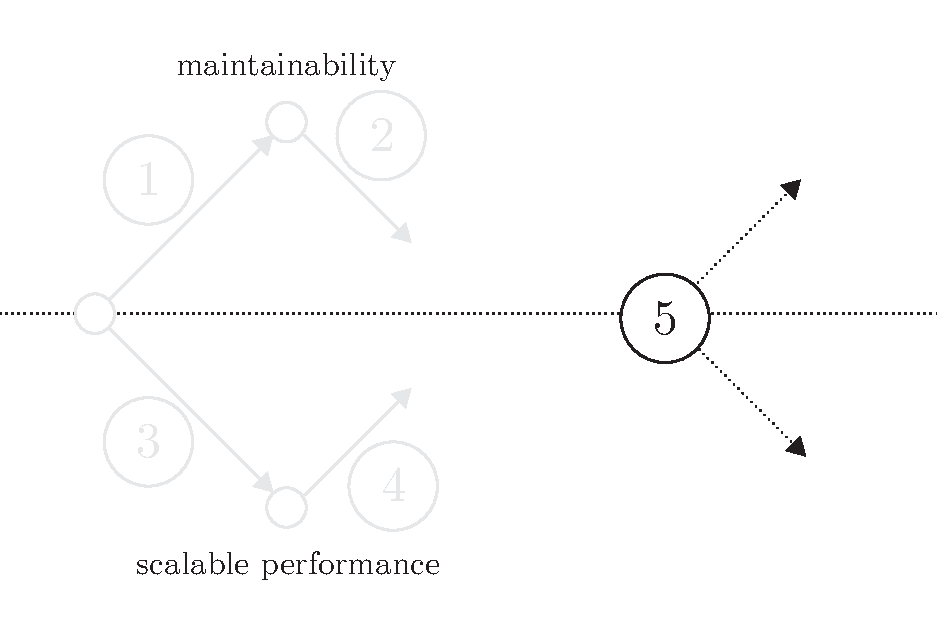
\includegraphics[width=0.6\textwidth]{../ressources/state-of-the-art-5.pdf}
\end{center}

The section \ref{chapter3:software-maintainability} shows that the modular organization enabled by functional programming is the best way to improve maintainability.
But it requires the use of a global memory store which conflicts with performance.
Compilation is a solution to reduce this conflict, but is not yet satisfactory enough for high performance scalability.
On the other hand, the section \ref{chapter3:software-performance} shows that to attain performance scalability, an application needs to multiply the exclusive accesses to its state.
That implies follow a distributed organization of its state to provide isolation and immutability, which negatively impacts modularity, hence maintainability.
Some works provide a uniform memory access to improve maintainability, despite the distributed execution.

The evolution of the economical constraints of a web application requires to repeatedly switch between maintainability and performance scalability.
The incompatibility between the two organizations implies technological ruptures at each switch.
Huge developing efforts are pulled to translate manually from one organization into the other, and later to maintain the implementation despites its unmaintainable nature.
There is still room for improvements on a compromise between maintainability and performance scalability.

The state of the art highlighted that
\begin{itemize}
\item maintainability requires lazy-evaluation and higher-order programming, section \ref{chapter3:software-maintainability:programming-models:functional-programming}, and
\item higher-order programming requires a global memory abstraction, section \ref{chapter3:software-maintainability:modular-programming:limitations},
\end{itemize}
Javascript is a functional language that features higher-order programming and a global memory abstraction.
% Moreover, its dynamic natures allows a lot of flexibility for the developers.
Moreover, node.js features a streaming approach with the event-loop execution model, similar to the lazy evaluation.
These reasons make Javascript a language of choice for developing web application.

And that
\begin{itemize}
\item scalable performance requires parallelism, and
\item parallelism requires exclusive accesses on the state through isolation and immutability.
\end{itemize}
Eventually, web development is heading toward a streaming approach with pipeline processing.

\nt{TODO dependency schema of these highlights}

This thesis proposes an equivalence between the global memory and control flow on one hand, and memory isolation with message passing on the other hand.
It proposes this equivalence as a solution to conciliate the scalable performance and maintainability.
As explained below, the concurrency model of the event-loop execution model, and the parallel approach of the pipeline execution model are very similar.
The goal of this thesis is to allow to compile one execution model into the other, to allow developers to constantly keep two organization of their implementation, allowing them to focus on both maintainability and scalable performance.

\subsection{Equivalence}

The next paragraphs introduces this equivalence between the event-loop execution model and the pipeline execution model.
The equivalence addresses two \textit{levels}\nt{not the good word}, as illustrated in figure \ref{fig:chapter3:objectives:roadmap}, the control flow, and the memory isolation.

\begin{figure}[h!]
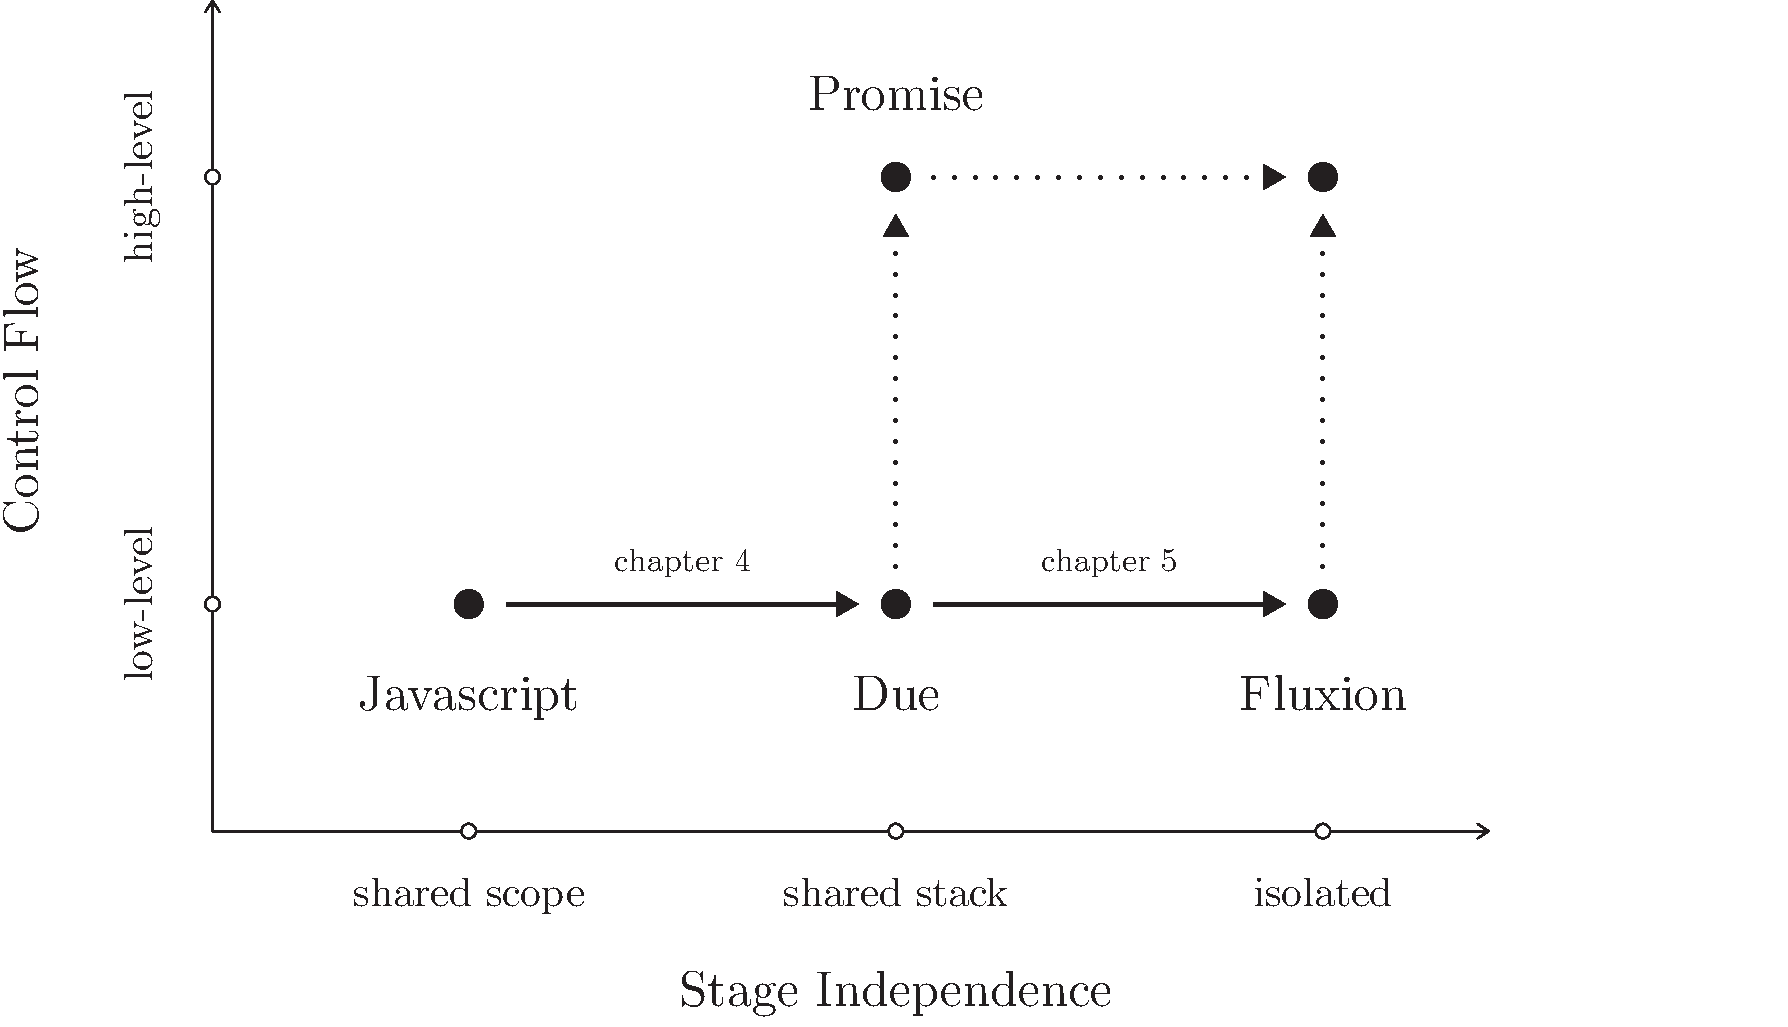
\includegraphics[width=1\textwidth]{../ressources/roadmap.pdf}
\caption{Roadmap}
\label{fig:chapter3:objectives:roadmap}
\end{figure}

\subsubsection{Rupture Point}

The execution of the pipeline architecture is well delimited in isolated stages.
Each stage has its own thread of execution, and is independent from the others.
On the contrary, the code of the event-loop is linear because of the continuation passing style and the common memory store.
% The message passing linking the callbacks is transparently handled by the event-loop.
However, the execution of the different callbacks are as distinct as the execution of the different stages of a pipeline.
The call stacks of two callbacks are distinct.
Therefore, an asynchronous function call represents the rupture between two call stacks.
It is a rupture point, and is equivalent to a data stream between two stages in the pipeline architecture.

Both the pipeline architecture and the event-loop present these rupture points.
The detection of rupture points allows to map a pipeline architecture onto the implementation following the event-loop model.
To allow the transformation from one to the other, this thesis studies the possibility to detect rupture points, and to distribute the global memory into the parts defined by these rupture points.
The detection of rupture points is addressed in chapter \ref{chapter4}.

It presents the extraction of a pipeline of operations from a Javascript application.
Indeed, such pipeline is similar to the one exposed by Promises.
The chapter proposes a simpler alternative to the latter called Dues.
However, these operations still require a global memory for coordination so they are not executed in parallel.

\subsubsection{Invariance}

% This transformation is important on two points.
% The conservation of the invariance.
% The equivalence between the coordinations.

The transformation should preserve the invariance as expressed by the developer to assure the correctness of the execution.
The partial ordering of events in a system, by opposition to total ordering, is sufficient to assure this correctness.
% This result was used by Lamport to prove the correctness of distributed systems.
The global memory is a way to assure the total ordering of events, and the message passing coordination is a way to assure partial ordering of events.
Therefore, to assure the correctness of the execution of a system, the state coordination with a global memory is equivalent to message passing coordination.
And it is possible, at least for some rupture points, to transform the global memory coordination into message passing while conserving the correctness of execution.

In order to preserve the invariance assured by the event-loop model after the transformation, each stage of the pipeline needs to have an exclusive access to memory.
The global memory needs not to be split into parts and distributed into each of the stages.
To assure the missing coordinations assured by the shared memory between the stages, the transformation should provide equivalent coordination with message passing.
The isolation and replacement of the global memory is fully address in chapter \ref{chapter5}, with the introduction of isolated containers called Fluxions.




% The invariance holds for the whole memory during the execution of each callback.
% As I explained in the previous section, this invariance is required to allow the concurrent execution of the different tasks.
% On the other hand, the invariance is explicit in the pipeline architecture, as all the stages have isolated memories.
% The coordination between these isolated process is made explicit by the developer through message passing.

% I argue that the state coordination between the callbacks requireing a global memory could be replaced by the message passing coordination used manually in the pipeline architecture.
% I argue that not all applications need concurrent access on the state, and therefore, need a shared memory.
% % Specifically, I argue that each state region remains roughly local to a stage during its modification.
% \nt{TODO review that, I don't know how to formulate these paragraphs. Identify the state and the data in the global memory.}

% \subsubsection{Transformation}

% This equivalence should allow the transformation of an event loop into several parallel processes communicating by messages.
% In this thesis, I study the static transformation of a program, but the equivalence should also hold for a dynamic transformation.
% I present the analyzis tools I developed to identify the state and the data from the global memory.




%-----------------------------------------------------------------------------%
                                    \endinput
%-----------------------------------------------------------------------------%


\section{Introduction}

In this section I analyze the current solutions to provide concurrency for web servers.
The criterion for this analysis are :

\begin{itemize}
\item how the solution (language) exposes the memory to the developer.
\item how the solution (language) exposes the invariance on this memory. These two language choices should be representative of the ease for a developer to develop with this language.
\item how the solution (infrastructure) finally extract parallelism based on the memory and its invariance (annotations or not, and how well ).
\item The expected ratio of parallelism over the total execution. and the ratio of communcation over the total state. These two ratios should be representative of the expected speedup in function of the resources made available.
\end{itemize}

We argue that the best solution is to provide a global memory to support software development practices, to provide an implicit invariance that the developer doesn't need to explictely define, like in transactional memory, lock, and so on ...
But yet provide parallelism for the execution to be scalable, with only a minimum of communication.

To lay the base for this analysis, I fisrtly present in more precision what is concurrency and scalability, and how it is studied in the litterature.
Then I analyze different solution to provide concurrency for web-applications.

\comment{The different solutions are roughly multi-process with message passing, multi-threading and the event-loop. I will detail this solution in greater details later.}

We analyze Javascript as an exammple in a class of higher-order languages using an event-loop with continuation passing style, for asynchronous programming.

% Section \ref{chapter3:javascript}
% Section \ref{chapter3:concurrency}
% Section \ref{chapter3:scalability}

% \section{Javascript}

\subsection{Explosion of Javascript popularity}

\subsubsection{In the beginning}

Javascript was created by Brendan Eich at Netscape around May 1995, and released to the public in September.
The initial name of the project was Mocha, then LiveScript, the name Javascript was finally adopted to leverage the trend around Java.
The latter was considered the hot new web programming language at this time.
It was quickly adopted as the main language for web servers, and everybody was betting on pushing Java to the client as well.
The history proved them wrong.
% Javascript slowly took over the client, and is now pushing toward the server.
% But that was not a calm and linear journey.

In 1995, when Javascript was released, the world wide web started its wide adoption.\ftnt{http://www.internetlivestats.com/internet-users/}
Browsers were emerging, and started a battle to show off the best features and user experience to attract the wider public.\footnote{to get an idea of the web in 1997 : \url{http://1x-upon.com/}}
Microsoft released their browser Internet Explorer 3 in June 1996 with a concurrent implementation of Javascript.
They changed the name to JScript, to avoid trademark conflict with Oracle Corporation, who owns the name Javascript.
The differences between the two implementations made difficult for a script to be compatible to both.
At the time, signs started to appear on web pages to warn the user about the ideal web browser to use for the best experience on this page.
This competition was fragmenting the web.
% and the overall user experience could be improved by /// according the technology ///.

To stop this fragmentation, Netscape submitted Javascript to Ecma International for standardization in November 1996.
In June 1997, ECMA International released ECMA-262, the first specification of ECMAScript, the standard for Javascript.
A standard to which all browser should refer for their implementations.
% TODO more on the Ecma specification ?

The base for this specification was designed in a rush. The version released in 1995 was finished within 10 days.
Because of this precipitation, the language has often been considered poorly designed and unattractive.
Moreover, Javascript was intended to be simple enough to attract unexperienced developers, by opposition to Java or C++, which targeted professional developers.
For these reasons, Javascript started with a poor reputation among the developer community.

But things evolved drastically since.
When a language is released, available freely at a world wide scale, and simple enough to be handled by a generation of teenager inspired by the technology hype, it produce an effervescent community around what is now one of the most popular and widely used programming language.

\subsubsection{Rising of the unpopular language}

Javascript started as a programming language to implement short interactions on web pages.
The best usage example was to validate some forms on the client before sending the request to the server.
This situation hugely improved since the beginning of the language.
So much that web-based, Javascript applications are currently now favored instead of rich, native desktop applications.

ECMA International released several version in the few years following the creation of Javascript.
The first and second version, released in 1997 and 1998, brought minor revisions to the initial draft.
However, the third version, released in the late 1999, contributed to give Javascript a more complete and solid foundation as a programming language.
From this point on, the consideration for Javascript keep improving.

An important reason for this reconsideration started in 2005.
James Jesse Garrett released \textit{Ajax: A New Approach to Web Applications}, a white paper coining the term Ajax \cite{Garrett2005}.
This paper point the trend in using this technique, and explain the consequences on user experience.
Ajax stands for Asynchronous Javascript And XML.
It consists of using Javascript to dynamically request and refresh the content of a web page.
The advantage is that it avoids to request a full page from the server.
Javascript is not anymore confined to the realm of small user interactions on a terminal, it can be proactive and responsible for a bigger part in the system spanning from the server to the client.
Indeed, this ability to react instantly to the user started to narrow the gap between web and native applications.
%, while keeping all the advantages of web-based applications.
At the time, the first web applications to use Ajax were Gmail, and Google maps\footnote{A more in-depth analysis of the history of Ajax, given by late Aaron Swartz \url{http://www.aaronsw.com/weblog/ajaxhistory}}.

Around this time, the Javascript community started to emerge.
The third version of ECMAScript had been released, and the support for Javascript was somewhat homogeneous on the browsers but far from perfect.
Moreover, Javascript is only a small piece in the architecture of a web-based client application.
The DOM, and the \texttt{XMLHttpRequest} method, two components on which AJAX relies, still present heterogeneous interfaces among browsers.
To leverage the latent capabilities of Ajax, and more generally of the web, Javascript framework were released with the goal to straighten the differences between browsers implementations.
Prototype\ftnt{http://prototypejs.org/} and DOJO\ftnt{https://dojotoolkit.org/} are early famous examples, and later jQuery\ftnt{https://jquery.com/} and underscore\ftnt{http://underscorejs.org/}.
These frameworks are responsible in great part to the wide success of Javascript and of the web technologies.

In the meantime, in 2004, the Web Hypertext Application Technology Working Group\ftnt{https://whatwg.org/} formed to work on the fifth version of the HTML standard.
This new version provide new capabilities to web browsers, and a better integration with the native environment.
It features geolocation, file API, web storage, canvas drawing element, audio and video capabilities, drag and drop, browser history manipulation, and many mores
It gave Javascript the missing pieces to become a true language for developing rich application.
The first public draft of HTML 5 was released in 2008, and the fifth version of ECMAScript was released in 2009.
With these two releases, ECMAScript 5 and HTML5, it is a next step toward the consideration of Web-based technologies as equally capable, if not more, than native rich applications on the desktop.
Javascript became the programming language of this rising application platform.

However, if web applications are overwhelmingly adopted for the desktop, HTML5 is not yet widely accepted as ready to build complete application on mobile, where performance and design are crucial.
Indeed web-technologies are often not as capable, and well integrated as native technologies.
But even for native development, Javascript seems to be a language of choice.
An example is the React Native Framework\ftnt{https://facebook.github.io/react-native/} from Facebook, which allow to use Javascript to develop native mobile applications.
They prone the philosophy \textit{"learn once, write anywhere"}, in opposition to the usual slogan \textit{"write once, run everywhere"}.\footnote{Used firstly by Sun for Java, but then stolen by many others}
% Another example is Gnome-shell. It uses Javascript to build its interface, and extensions.
% PhoneGap (Cordova) is a huge effort toward bringing web technologies to the mobile. 

\subsubsection{Current situation}

\cit{When JavaScript was first introduced, I dismissed it as being not worth my attention. Much later, I took another look at it and discovered that hidden in the browser was an excellent programming language.}{Douglas Crockford}

% \cit{JavaScript is the world's most ubiquitous computing runtime.}{John Lam}

The success of Javascript is due to many factors ; I mentioned previously the standardization, Ajax libraries and HTML5.
Another factor, maybe the most important, is the View Source menu that reveals the complete source code of any web application.
\textit{The view source menu is the ultimate form of open source}\ftnt{http://blog.codinghorror.com/the-power-of-view-source/}.
It is the vector of the quick dissemination of source code to the community, which picks, emphasizes and reproduces the best techniques.
This brought open source and collaborative development before github. \comment{TODO neither open source nor collaborative development are the correct terms}
Moreover, all modern web browsers now include a Javascript interpreter, making Javascript the most ubiquitous runtime in history \cite{Flanagan2006}.
% Every browser include development tools for Javascript, making it the most ubiquitous development environment, as well.

When a language like Javascript is distributed freely with the tools to reproduce and experiment on every piece of code.
When this distribution is carried during the expansion of the largest communication network in history.
Then an entire generation seizes this opportunity to incrementally build and share the best tools they can.
This collaboration is the reason for the popularity of Javascript on the Web.

% I want to say that Javascript took off because it was carried by the open source community.
% The goal is to introduce the following facts : JS is widely used in the open source community.
% I need to find the argument saying that open source is taking over closed sources : Javascript / open source is taking over Java / closed source.

% TO READ :
% http://www.javaworld.com/article/2077224/learn-java/is-javascript-here-to-stay-.html
% http://blog.codinghorror.com/the-power-of-view-source/
% http://blog.codinghorror.com/javascript-the-lingua-franca-of-the-web/
% http://shaver.off.net/diary/2007/05/10/the-high-cost-of-some-free-tools/


% This success is obvious on the web and in the open source communities.
It seems to also infiltrate many other fields of IT, but it is hard to give an accurate picture of the situation.
There is no right metrics to measure programming language popularity.
In the following paragraphs, I report some popular metrics and indexes available on the net.
More detailed informations are available section \ref{appendix:langpop}.

\paragraph{Search engines}

The TIOBE Programming Community index is a monthly indicator of the popularity of programming languages.
It uses the number of results on many search engines as a measure of the activity of a programming language.
Javascript ranks 6th on this index, as of April 2015, and it was the most rising language in 2014.
However, the measure used by the TIOBE is controversial.
Some says that the measure is not representative.
It is a lagging indicator, and the number of pages doesn't represent the number of readers.

On the other hand, the PYPL index is based on Google trends to measure the activity of a programming language.
Javascript ranks 7th on this index, as of May 2015.

From these indexes, the major programming languages are Java, C/C++ and C\#.
The three languages are still the most widely taught, and used to write softwares.
But Javascript is rising to become one of these important languages.

\paragraph{Developers collaboration platforms}

Github is the most important collaborative development platform, with around 9 millions users.
Javascript is the most used language on github since mid-2011, with more than 320 000 repositories.
The second language is Java with more than 220 000 repositories.

\comment{TODO : graph of Github repositories by languages}

StackOverflow, is the most important Q\&A platform for developers.
It is a good representation of the activity around a language.
Javascript is the second language showing the most activity on StackOverflow, with more than 840 000 questions.
The first one is Java with more than 850 000 questions.

Black Duck knowledgebase analyzes 1 million repositories over various forges, and collaborative platforms to produce an index of the usage of programming language in open source communities.
Javascript ranks second.
C is first, and C++ third.
Along with Java, the four first languages represent about 80\% of all programming language usage.

% TODO redo this graph, it is ugly.
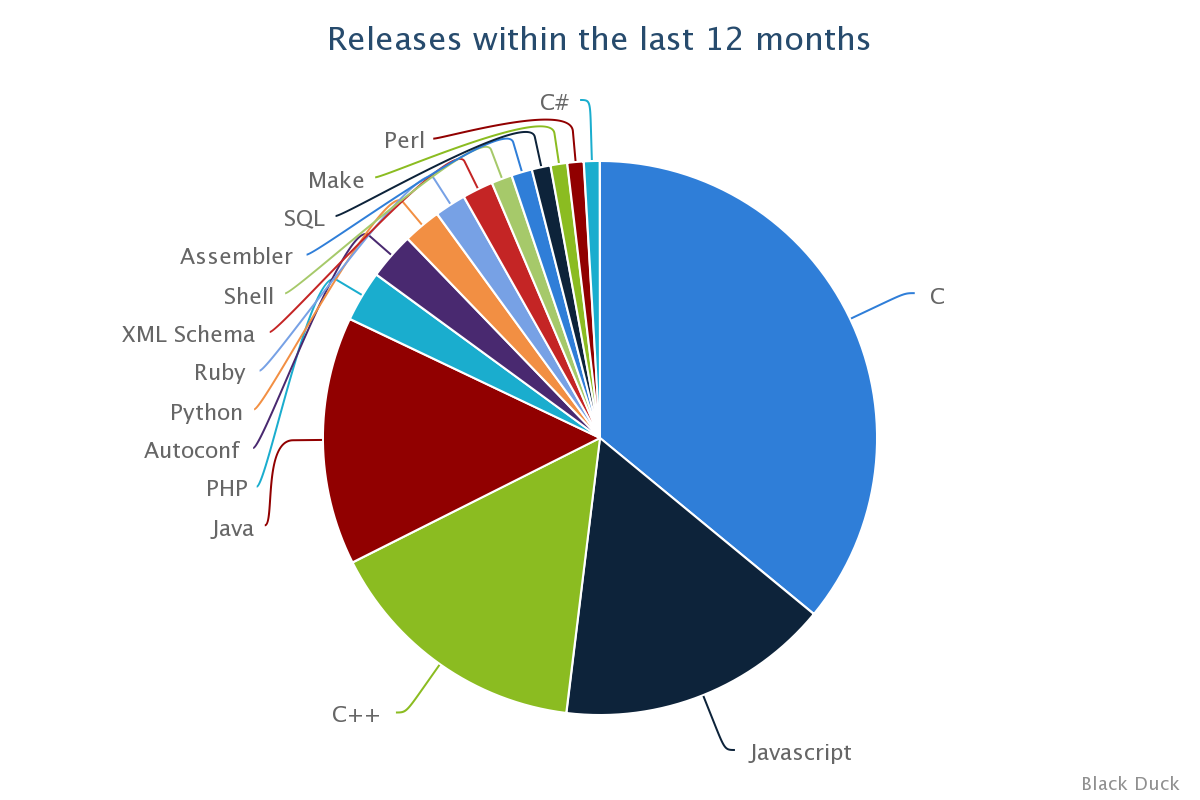
\includegraphics[width=0.9\linewidth]{../../data/js-trends/black-duck-15}

\paragraph{Jobs}

All these metrics are representing the visible activity about programming language.
But not the entire software industry is open source, and the activity is rather opaque.
To get a hint on the popularity of programming languages used in the software industry, let's look at the job offerings.
Indeed provide some insightful trends.
Javascript developers ranked at the third position, right after SQL developers and Java developers.
Then come C\# and C developers.

% TODO redo this graph, it is ugly.
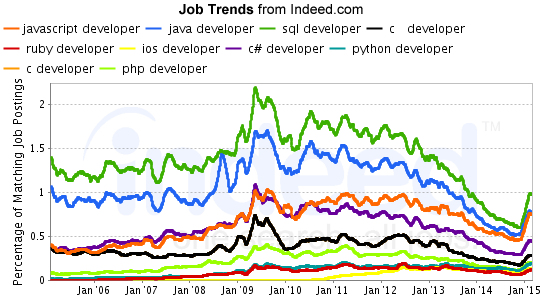
\includegraphics[width=0.9\linewidth]{../../data/js-trends/jobgraph}

All these metrics represent different faces of the current situation of Javascript adoption.
We can safely say that Javascript is one of most important language of this decade, along with Java, C/C++.
It is widely used in open source projects, and everywhere on the web.
But it is also trending, and maybe slowly replacing languages like Java.
% TODO continue this

\paragraph{Future trends}

\comment{TODO}

Code reuse.
Why it never worked ?




\comment{em-scripten}

https://github.com/kripken/emscripten
Javascript is a target language for LLVM, therefor everything can compile to Javascript : JS is the assembler of the web.

\comment{Isomorphic Javascript}

Server-side Javascript

https://www.meteor.com/
https://facebook.github.io/flux/
Javascript can be executed both on the client and the server.
That allow use-cases never possible before (server pre-rendering, same team ...)

\comment{Reactive}

http://facebook.github.io/react/
Javascript is used to model the flow of propagation of state in a web application



---

Some facts to include :
https://www.destroyallsoftware.com/talks/the-birth-and-death-of-javascript
The Atom editor is written in Javascript node.js.
Now, major PaaS (which one) support node.js by default.
Heroku support Python, Java, Ruby, Node.js, PHP, Clojure and Scala
Amazon Lambda Web service support node.js in priority.
npm raises 8m.
http://techcrunch.com/2015/04/14/popular-javascript-package-manager-npm-raises-8m-launches-private-modules/

% >>> I want to say that Javascript is now broadly used.
% Let's just look at the numbers : Javascript is the most popular language on Github, and npm has more package than any other package manager.
% Javascript has the more broadly deployed runtime.
% ... and so on
% >>> the conclusion is : Javascript is now a major language, and it is more than worth the consideration we are giving it in this PhD thesis.

\subsection{Overview of the language}

Javascript was released in a hurry, without a strong and directive philosophy.
During its evolution, it snowballed with different features to accommodate the community, and the usage it was made on the web. As a result Javascript contains various, and sometimes conflicting, programming paradigms.
It borrow its syntax from a procedural language, like C, and the object notation from an object-oriented language, like Java, but it provides a different inheritance mechanism, based on prototypes. Most of the implementation adopt an event-based paradigm, like the DOM\ftnt{http://www.w3.org/DOM/} and node.js\ftnt{https://nodejs.org/}.
And finally, event though it is not purely functional like Haskel, Javascript borrows some concepts from functional programming.

In this section, we focus on the last two programming paradigm, functional programming and event-based programming.
Javascript exposes two features from functional programming that are particularly adapted for event-based programming.
Namely, it treats functions as first-class citizen, and allows them to close on their defining context, to become closures.
% TODO In the next section, we explain this two features
% TODO and in the second section, we explain event-based programming and why these two features are good for event-based programming

\subsubsection{Functions as First-Class citizens}

\cit{All problems in computer science can be solved by another level of indirection}{Butler Lampson}

Javascript treats function as first-class citizens.
One can manipulate functions like any other type (number, string ...).
She can store functions in variables or object properties, pass functions as arguments to other functions, and write functions that return functions.

The most common usage examples of these features, are the methods \texttt{Map}, \texttt{Reduce} and \texttt{filter}.
In the example below, the method \texttt{map} expect a function to apply on all the element of an array to modify its content, and output a modified array.
A function expecting a function as a parameter is considered to be a higher-order function. \texttt{Map}, \texttt{Reduce} and \texttt{Filter} are higher-order functions.

\begin{code}
  [4, 8, 15, 16, 23, 42].map(function firstClassFunction(element) {
    return element + 1;
  });
  // -> [5, 9, 16, 16, 24, 43]
\end{code}

Higher-order functions provide a new level of indirection, allowing abstractions over functions.
To understand this new level of abstraction, let's briefly summarize the different abstractions on the execution flow offered by programming paradigms.
In imperative programming, the control structures allow to modify the control flow. That is, for example, to execute different instructions depending on the state of the program.
Procedural programming introduces procedures, or functions. That is the possibility to group instructions together to form functions.
They can be applied in different contexts, thus allowing a new abstraction over the execution flow.
% It encourages to abstract program states so that the same function can be applied in different places to apply its behavior.

So, higher-order functions add another level of abstraction.
It allows to dynamically modify the control of the execution flow.
The ability to manipulate functions like any other value allows to abstract over functions, and behavior.
% TODO continue this, there is a lot to say about HOF

Higher-order functions replace the needs for some Object oriented programming design patterns.\ftnt{http://stackoverflow.com/a/5797892/933670} Though object oriented programming doesn't exclude higher-order functions.

They are particularly interesting when the behavior of the program implies to react to inputs provided during the runtime, as we will see later.
Web servers, or graphical user interfaces, for examples, interact with external events of various types.

% TODO transition : higher-order functions makes use of closure to implement the lexical scope in mutable programming languages. (reformulate)

\subsubsection{Lexical Scoping}

Closures are indissociable from the concept of lexical environment.
To understand the former, it is important to understand the latter first.

\paragraph{Lexical environment}

A variable is the very first level of indirection provided by programming languages and mathematics.
It is is a binding between a name and a value.
Mutable like in imperative programming to represent the reality of memory cells, or immutable like in mathematics and functional programming.
These bindings are created and modified during the execution.
They form a context in which the execution takes place.
To compartmentalize the execution, a context is also compartmentalized.
A certain context can be accessed only by a precise portion of code.
Most languages defines the scope of this context using code blocks as boundaries.
That is known as lexical scoping, or static scoping.
The variables declared inside a block represent the lexical environment of this block.
These lexical environments are organized following the textual hierarchy of code blocks.
The context available from a certain block of code, that is set of accessible variable, is formed as a cascade of the current lexical environment and all the parent lexical environment, up to the global lexical environment.

% TODO draw the schema for a lexical environment here

\paragraph{Javascript lexical environment}
\ftnt{http://www.ecma-international.org/ecma-262/5.1/\#sec-10.2}

Javascript implement lexical scoping with function definitions as boundaries, instead of code blocks.
The code below show a simple example of lexical scoping in Javascript.

\begin{code}
  var a = 4;
  var c = 6;
  function f() {
    var b = 5;
    var c = 0;
    // a and b are accessible here.
    return a + b + c;
  }

  f(); // -> 9

  // b is not accessible here :
  a + b + c; // -> ReferenceError: b is not defined
\end{code}

Lexical scoping, or statical scoping, implies that the lexical environment are known statically, at compile time for example.
But Javascript is a dynamic language, it doesn't truly provide lexical scoping.
In Javascript, the lexical environments can be dynamically modified using two statements : \texttt{with} and \texttt{eval}.
We explain in details the Javascript lexical scope in section \ref{??? Compiler stuff}

\subsubsection{Closure}

\cit{An object is data with functions. A closure is a function with data.}{John D. Cook}

A closure is the association of a first-class function with its context.
When a function is passed as an argument to an higher-order function, she closes over its context to become a closure.
When a closure is called, it still has access to the context in which it was defined.
The code below show a simple example of a closure in Javascript.
The function \texttt{g} is defined inside the scope of \texttt{f}, so it has access to the variable \texttt{b}.
When \texttt{f} return \texttt{g} to be assigned in \texttt{h}, it becomes a closure.
The variable \texttt{h} holds a closure referencing the function \texttt{g}, as well as its context, containing the variable \texttt{b}.
The closure \texttt{h} has access to the variable \texttt{b} even outside the scope of the function \texttt{f}.

\begin{code}
  function f() {
    var b = 4;
    return function g(a) {
      return a + b;
    }
  }

  var h = f();
  // b is not accessible here :
  b; // -> ReferenceError: b is not defined

  // h is the function g with a closure over b :
  h(5) // -> 9
\end{code}


% TODO continue with closure


% TODO transition, Higher-order functions and closures are very handy in turn-based programming.
% Turn based programming is the programming model of the event-loop, which is the concurrent model for I/O bound applications.
% \section{Concurrency}


% http://berb.github.io/diploma-thesis/original/043_threadsevents.html

% On the Duality of Operating System Structures
% http://tolstenko.net/blog/dados/Unicamp/2010.1/mc714/extras/201_recomendada_Lauer-Needham-78-Duality.pdf

% Threads vs. Events
% http://courses.cs.vt.edu/cs5204/fall09-kafura/Presentations/Threads-VS-Events.pdf

% Why Threads Are A Bad Idea (for most purposes)
% http://www.cs.utah.edu/~regehr/research/ouster.pdf

% Why Events Are A Bad Idea (for high-concurrency servers)
% http://static.usenix.org/publications/library/proceedings/hotos03/tech/full_papers/vonbehren/vonbehren_html/

% http://www.usingcsp.com/cspbook.pdf

% Threads Without the Pain
% http://queue.acm.org/detail.cfm?id=1105678


% Cooperative Task Management without Manual Stack Management or, Event-driven Programming is Not the Opposite of Threaded Programming 
% http://static.usenix.org/publications/library/proceedings/usenix02/full_papers/adyahowell/adyahowell_html/

% Retrospective on SEDA
% http://matt-welsh.blogspot.fr/2010/07/retrospective-on-seda.html

% Latency
% http://highscalability.com/latency-everywhere-and-it-costs-you-sales-how-crush-it
% http://blog.gigaspaces.com/amazon-found-every-100ms-of-latency-cost-them-1-in-sales/




\subsection{About concurrent systems}

This demonstration focus on application depending on long waiting operations like I/O operations.
Particularly, this demonstration focus on real-time web services.
It is irrelevant for application heavily relying on CPU operations, like scientific applications.

Threads-based system and event-based system evolved significantly over the last half century.
These evolutions were fueled by the long-running debate about which design is better.
We try to succinctly and roughly retrace theses evolutions to understand the positions of each community.
This demonstration show that thread and events are two faces of the same reality.

Lauer and Needham \cite{Lauer1979} presented an equivalence between Procedure-oriented Systems and a Message-oriented Systems.

% TODO brief historic


Adya \textit{et. al.} analyzed this debate and presented fives categories through which to present the problem \cite{Adya2002}.
These two categories were often associated with thread-based systems and event-based systems.
% TODO not very clear
Their advantages and drawbacks were mistaken with those of thread and events.
Adya \textit{et. al.} explain in details two of these categories that are most representative, Task management and Stack management.
We paraphrase these explanations.

\subsubsection{Task management}

Consider a task as an encapsulation of part of the logic of a complete application.
All the task access the same shared state.
The Task management is the strategy chosen to arrange the task executions in available space and time.

Preemptive task management executes each task concurrently.
Their executions interleave on a single core, or overlap on multiple cores.
It allows to leverage the parallelism of modern architectures.
This parallelism has a cost however, developers are responsible for the synchronization of the shared memory.
While accessing a memory cell, it must be locked so that no other task can modify it.
Synchronization mechanism impose the developer to be especially aware of race condition, and deadlocks.
These synchronization problems make concurrency hard to program with preemptive task management.

The opposite approach, Serial task management, executes each task to completion before starting the next.
The exclusivity of execution assures an exclusive access on the memory.
Therefore, it removes the need for synchronization mechanism.
However, this approach is ill-fitted for modern applications, where concurrency is needed.

A compromise approach, Cooperative task management, allows tasks to yield voluntarily.
A task may yield to avoid monopolizing the core for too long.
Typically, it yields to avoid waiting on long I/O operations.
It merges the concurrency of the preemptive task management, and the exclusive memory access.
Thus, it relieves the developer from synchronization problems.
But at the cost of dropping parallel execution.

Threads are associated with preemptive task management, and events with Cooperative task management.
For this reason, it is commonly believed that synchronization mechanisms make threads hard to program \cite{Ousterhout1996}.
While it is really Preemptive task management that is responsible for these synchronization problems \cite{Adya2002}.

% TODO define the two
\subsubsection{Stack management}

Consider a task is composed of several subtasks interleaved with I/O operations.
Each I/O operation signal its completion with an event.
The task stops at each I/O operation, and must wait the event to continue the execution.
The stack management is the strategy chosen to express the sequentiality of the subtasks.

The automatic stack management is what is mostly used in imperative programming.
The execution seems to wait the end of the operations to continue with the next instruction.
The call stack is kept intact.
This is what is commonly called synchronous programming.

In the manual stack management, developers need to manually register the handlers to continue the execution after the operation.
The execution immediately continues with the next instruction, without waiting the completion of the operation.
It implies to rip the call stack in two functions; one to initiate the operation, and another to retrieve the result.
This is what is commonly called asynchronously programming.

% TODO advantage and disadvantages of synchronous and asynchronous programming

What we argue is that synchronous is good because it is linear, it avoids stack ripping.
But asynchronous is good because it allows parallelism by default.


% synchronous programming is good to express linear execution. In parallel that means quite unrelated linear executions.
% asynchronous programming is good to express interleaved parallel execution. It is easy to express small parallel and sequential tasks.


Threads are associated with the automatic stack management, and events with manual stack management.
For this reason, it is commonly believed that threads are easier to program.
\cite{Thread systems allow programmers to express control flow and encapsulate state in a more natural manner} \cite{Behren2003}.
However, the automatic stack management is not exclusive to threads.
Fibers, presented by Adya \textit{et. al.} is an example of cooperative task management with automatic stack management \cite{Adya2002} .
Fibers present the advantage of cooperative task management, without the disadvantage of stack ripping.
That is the ease of programming because of the absence of synchronization, without the difficulty of stack ripping.

We argue that the advantages of manual stack management outweigh its drawbacks for web services.
Because of the numerous I/O operations, parallelism is 


% TODO I split the explenation in thread then events, instead, I should split in task management, then state management




But what is actually highlighted is the automatic state management provided by threads.
And with lighter context change, threads are a good choice which provide parallelism.

Historically, events-based system are associated with manual state management, while threads-based systems are associated with automatic state management.
Manual state management imposed stack ripping \cite{Adya2002}.
With closure, it is not the case anymore.
Events now have automatic state management as well \cite{Krohn2007}.

Now, there is implementation of thread model with cooperative management, with context-switch overhead improved enough to fill the gap with events model.
And there is implementation of event model with automatic state management filling the gap with thread model.
In this condition, we ask, what really is the difference between thread and events.
We argue there is none.
Except the isolation, versus sharing of the memory, which, again is not significant of either.
In the first case, the different execution threads exchange messages, while in the second, they use synchronization mechanism to assure invariants in their states % TODO disambiguation thread is a context for execution, what is a core of execution ?

For a single thread of execution, both model could avoid synchronization through cooperative task management, which assure invariants. % TODO disambiguation
Or avoid procedure slicing (if any) using synchronization.
These are the two ends of a design spectrum.
One end (cooperative task management) fits better for small processing with heavy use of shared resources.
While the other end (synchronization) fits better for long processing with small use of shared resources.
When one end of the design spectrum is used while the other should be used, one might expect unresponsiveness because of too heavy events, or performance fall due to interlocking.

Scalability is achieved through parallelism, which is itself achieved in our case (web servers) through cluster of commodity machines.
% TODO this links exactly to what I wrote on scalability, find a way to merge the two.

With distribution, this design spectrum gets a better contrast. % TODO that is really false, reformulate to get a correct articulation

The synchronization of distributed, shared resources is limited through the CAP theorem  \cite{Gilbert2002a}. % TODO needs to read this.
Partition tolerance is a requirement of a distributed system. %TODO define PA, and find reference http://codahale.com/you-cant-sacrifice-partition-tolerance/#ft2
One needs to choose good latency (availability) or consistency. % Define the CAP theorem, consistency and availability
The CAP theorem is generalized into a broader theroem about\cite{Gilbert2012} % TODO read, and merge within the argumentation (the paper seems really broad, be careful not to dive too deep)

The isolation of resources implies to split the architecture in different stages, like Ninja \cite{Gribble2001}, SEDA \cite{Welsh2000}, or Flash \cite{Pai1999}.
This splitting is difficult for the developer.
The splitting which is good for the machine, is not the same as the one good for the design in modules.

The two ends of this design spectrum presented map directly onto the two kinds of parallelism advocated for scalability.
That is pipeline parallelism, and data parallelism.

Pipeline parallelism is good for data locality, and important throughput. % TODO reference
But each stage adds an overhead in latency. % TODO reference

Data parallelism is good for latency, because one request is processed from beginning to the end without waiting in queues.
But it implies that the different machines share a common database.
Which is a shared resource, and is limited by the CAP theorem.

Both parallelism have advantages and drawbacks, and both could be combined, like in the SEDA architecture. % TODO find the exact reference that says : it is good to use both parallelism to scale
Ultimately, it would be possible to design a design spectrum to choose which kind of parallelism for a set of requirements.
But we leave this for future works.

Splitting an architecture in stages is a difficult process, which prevent future code refactoring, and module modifications.
We argue that the design for the technical architecture, and the design for the human minds should not be the same.
Threads belong to the mental model, the design granularity
Events belong to the execution model, the architecture granularity
  % TODO quote
  It is a mistake to attempt high concurrency without help from the compiler \cite{Behren2003}.
Through compilation, we want to transform an event-loop based program (cooperative task management, no synchronization) into a pipeline parallelism distributed system.
So, basically, we argue that it is possible to distribute one loop event onto multiple execution core.



% TODO Careful, you don't know fibers enough.
% And globally, there is much that you don't know.

% Il y à quelques années, la tendance chez les gros était de se concentrer sur la parallélisation par threads pour gagner en latence.
% Notamment avec Gigaspace.
% Donc en occultant complètement les events, et en utilisant des grosses bases de données comme Dynamo ou Cassandra qui scalent bien.
% Je n'ai pas vraiment trouvé la même tendance pour les events.
% Storm et Spark stream sont à usage plus spécifique.
% Mais ce déséquilibre est peut être simplement dû à l'héritage de l'architecture n-tier.


% MICROSERVICES
% Plus récemment, j'ai trouvé beaucoup de bruit sur les microservices en 2014.
% Ça me paraissait intéressant, en pensant y trouver des arguments pour favoriser les events, et nuancer la tendance précédente.
% Mais j'ai l'impression qu'il s'agit plus d'une question d'organisation humaine que de performance.
% Il me reste à trouver des arguments pour mettre à égalité les deux axes de parallélisation.





% TODO 
% Continue with the hybrid approach : multiple threads for events, and one threads for user code
% See Flash, SEDA, Node.js etc ...






/!\ WARNING
The paper Why events are a bad idea states that :
the control flow patterns used by these applications fell into three simple categories: call/return, parallel calls, and pipelines.
Indeed, it is no coincidence that common event patterns map cleanly onto the call/return mechanism of threads. Robust systems need acknowledgements for error handling, for storage deallocation, and for cleanup; thus, they need a “return” even in the event model.
>> Why is it completly false ?
	 It is crucial to find an answer.
Moreover, Ayda et. al. state that :
For the classes of applications we reference here [file servers and web servers], processing is often partitioned into stages.
Other system designers advocated non-threaded programming models because they observe that for a certain class of high-performance systems [...] substantial performance improvements can be optained by reducing context switching and carefully implementing application-specific cache-conscious task scheduling.


The paper Why events are a bad idea states that :
One could argue that instead of switching to thread systems, we should build tools or languages that address the problems with event systems (i.e., reply matching, live state management, and shared state management). However, such tools would effectively duplicate the syntax and run-time behavior of threads.
>> Well, yes ...
   With the exception of the stack junction.
   The paper on Duality had it right, their graph is correct, but for threads, it cannot be distributed because of stacks, while for events, it can.


Software evolution substantially magnifies the problem of function ripping: when a function evolves from being compute-only to potentially yielding, all functions, along every path from the function whose concurrency semantics have changed to the root of the call graph may potentially have to be ripped in two. (More precisely, all functions up a branch of the call graph will have to be ripped until a function is encountered that already makes its call in continuation-passing form.) We call this phenomenon ``stack ripping'' and see it as the primary drawback to manual stack management. Note that, as with all global evolutions, functions on the call graph may be maintained by different parties, making the change difficult. 
>> Stack ripping is what I am talking about.
   While the stack are joined, it is not possible to distribute.
   If they say that stack ripping is necessary, that means it is not possible to encapsulate asynchronous function into synchronous function.
% \section{Scalability}

% TODO introduction to this chapter


We define a web service as a computer program whose main interface is based on web protocols, such as HTTP.
Such a service uses resources allocated on a network of computers.
Scalability defines the ability of the service to use a certain quantity of resource to meet a desired performance.
We call system the association of the computer program and the available resources. 
The performance of this system is measured by its latency and throughput.

\subsection{Latency and throughput}

Latency is the time elapsed between the reception of a request, and the sent of the reply.
It includes the time waiting for resources to be free to process the request, and the time to process the request.

Throughput is the number of requests processed by the system by unit of time.

Latency and throughput are linked in a certain way.
If a modification of the web service reduces its mean latency to a half, then the throughput doubles immediately.
It takes half the time to process a request, therefore, the service can process more requests in the same time.
However, if throughput augment, the latency doesn't necessarily decrease.

\subsection{Scalability granularity}

We define a computer program as a set of operations.
In the case of a web service, these operations can be directly requested by the user through the interface.
An operation can cause any other operation to execute.

Because both the resources used and the operations executed are discrete : not infinitely divisible, scalability is inherently discrete.


% TODO scalability granularity ? 
Scalability granularity is the increment of resources.
How the input data can be split up ?
How the program can be deployed on many machines ?






We call system the association of the computer program with the resources


\subsection{Horizontal and vertical scaling}

There is two ways to augment the resources of the system.
Enhance the nodes in the computer network - vertical scaling.
Or add more nodes to the computer network - horizontal scaling.


% TODO how to apply these theory to highly concurrent servers ?
% How does it modify the theories ?

There are three theories, from the most restrictive, to the most general.


% TODO define scalability
Scalability is the property of a computer program to occupy available resources to meet a needed performance.
EIther in Latency, or in throughput.







\subsection{Linear scalability}

Clements et. al. \cite{Clements2013a} prove that a computer program scale linearly if all its operations are commutative.
% Commutative is not parallel. How to go from commutative to parallel ?
Two operations are said to be commutative if they can be executed in any orders, and the same initial state will result in the same final state.
Commutativity implies the two operations to be memory-conflict free, or independent, which is equivalent to say that they can be executed in parallel.

Therefore, to achieve linear scalability, a computer program must be composed of a set of operations that commutes.
Thus, all the operations are parallel, they can be executed simultaneously, on any number of machines as required.

The size of the operations sets the scalability granularity.

However, commutativity is not achievable in real applications.
Even sv6, the operating system resulting from the work on commutative scalability only has 99\% commutativity.
For real application, in the best case, the granularity is coarse, in the worst case, there is no possible commutativity because of shared resources (like a product inventory, or a friend graph).

% TODO continue

\subsection{Limited scalability}

Amdahl introduced in 1967 a law to predict the limitation of speedup a computer program can achieve if a fraction of its code is sequential.
Amdahl worked at increasing the speed of computer clock, while the scientific community was working on improving parallelism of computing machines.

In a set of operations, even if one is non-commutative, it cannot be executed in parallel of any others, the scalability is limited by this operation.

There is a difference if the operation is non-commutative with itself, or only with others.
In the first case, it impose a queuing, while in the second case, it only increase the granularity : you can regroup the non-commutative operation with its subsequents, and form a bigger commutative operation.

% TODO continue

\subsection{Negative scalability}

Gunther generalized Amdahl's law into the Universal Scalability Law.
It includes the parallelization of non-independent operations with the use of synchronization.

It models the negative return on scalability from sharing resources observed in many real world applications.

% TODO continue by explaining the different area of scalability.



\subsection{Eventual Consistency}

To overpass the scalability limits set by the previous rules, it is possible to abandon consistency.
It simply tolerate incoherences between multiple replicas.
The output of an operation can be false while its state is synchronized with the other replicas.

% It is similar to the propagation of sound, light or gravity.
% When an explosion happens, not everybody hears it at the same time : there is inconsistency in the experience.


% TODO continue

% \section{Framworks for web application distribution}
% \subsection{Micro-batch processing}
% \subsection{Stream Processing}

% \section{Flow programming}
% \subsection{Functional reactive programming}
% \subsection{Flow-Based programming}

% \section{Parallelizing compilers}
% \comment{OpenMP and so on}
% %\subsubsection{\comment{TODO}}

% \section{\comment{Synthesis}}
% \comment{There is no compiler focusing on event-loop based applications}


%-----------------------------------------------------------------------------%
                                    \endinput
%-----------------------------------------------------------------------------%

Objective
---------

My objective is to find a solution to allow a first code base to evolve continuously in performance. That is to avoid the rupture that is so often observed in the industry currently (e.g. LinkedIn, Facebook ... ).

I want to achieve that with a solution to transition from the imperative model presenting certain characteristics to a distributed model with certain conditions.

Cartography
-----------


# Industry -> We want to decrease development time while increasing performance. We barely care about used resources.

## Languages, libraries and frameworks

  + Java - Object-oriented
  +> Spring
  +> Scala - Functional + Object-oriented
  +>> Akka - Message driven actors
  +>>> Play - on top of akka (Asynchronous)

  + PHP - Object-oriented
  +> Sinatra

  + Ruby - Functional + Object-oriented
  +> Rails

  + Javascript - Functional + Prototype-oriented
  +> Express.js
  +> hapi.js
  +> Meteor
  +> Bacon.js - Reactive programming
  +> kraken.js

  + NoFlo

  + Haskell
  +> FRP Reactive programming

  + Spidle: A DSL approach to specifying streaming applications dataflow like

  + Erlang

## Databases

  + FlockDB
  + CouchDB
  + PouchDB
  + Cassendra
  + Dynamo DB

  + unhosted
  + MoveMyData

## Runtime

  + Node.js - Asynchronous programming with Event-loop
  +> Fibers 


# Embedded -> We want to decrease used resources while increasing performance. We barely care about development time.



+ Exploiting Coarse-grained Task, Data and Pipeline Parallelism in Stream Programs -> Compile StreamIt to assembler for multi-core

+ Shangri-La - Compile C-like into assembler for packet program

+ SPUR - A programming model for an embedded media processing architecture


# Scientific-like -> We want to increase performance. We barely care about used resources nor decreasing development time.

## Languages, libraries and frameworks

  + OpenMP
  + OpenCL
  + CUDA
  + Cg: A system for programming graphics hardware in a C-like language
  + Brook for GPUs: Stream Computing on Graphics Hardware
  + Liquid Metal by IBM - unified language for FPGAs, GPUs and such ...

  + StreaMIT: A language for Streaming Applications


  + Apache Kafka - publish/subscribe distributed commit log

  Design methodology:
  + PCAM - Partition -> Communicate -> Agglomerate -> Map

## Runtime

  + Vert.X - node like + thread / worker capabilities

  OSs :

  + BarrelFish
  + TesselationOS
  + Mosix
  + CoreOS


  Architectures:


    Web service oriented:
      Threads only:
      + Capricio - User cooperative threads (also known as fibers / green threads)

      Events only:
      + TAME - event-based solution without stack ripping in C (it is like closure, but for C)

      Hybrid solutions:
    + AMPED Asymetric multi-process event-driven
    +> Flash
    +> Nginx
    +> Ninja
    +> SEDA
    +> Leda - PCAM 
    + Combining events and threads for scalable network services, Linguistic symbiosis between event loop actors and threads, Combining data flow and control flow computing)

    + 

    + Cluster-based scalable network services


  + Grape / Timestream - distributed SQL (roughly)
  + CQL
  +> STREAM (uses CQL)
  + StreaQuel
  +> TelegraphCQ
  + AQuery

  (From the paper : Making state explicit for imperative big data processing)
  + MapReduce       map/reduce   |   Stateless dataflow
  + DryadLINQ       functional   |   Stateless dataflow
  + Spark           functional   |   Stateless dataflow
  + CIEL            imperative   |   Stateless dataflow
  + Hadoop          map/reduce   |   Stateless dataflow
  + Incoop          map/reduce   |   Incremental dataflow
  + Nectar          functional   |   Incremental dataflow
  + CBP             dataflow     |   Incremental dataflow
  + Comet           functional   |   Batched dataflow
  + D-Streams       functional   |   Batched dataflow
  + Naiad           Dataflow     |   Batched dataflow
  + Storm, S4       dataflow     |   Continuous dataflow
  + SEEP            dataflow     |   Continuous dataflow
  + Piccolo         imperative   |   Parallel in-memory
  + SDG             imperative   |   Stateful dataflow




What about all the techniques for analyzing and extracting parallelism :

+ Commutativity analysis: a new analysis technique for parallelizing compilers
+ the scalable commutativity rule ...
+ Making asynchronous parallelism safe for the world


+ Cooperative task management without manual stack management - Hybrid approach, fibers + threads




- transactional memory
  - http://www.morganclaypool.com/doi/abs/10.2200/s00272ed1v01y201006cac011
  - http://delivery.acm.org/10.1145/1370000/1364800/p80-larus.pdf?ip=160.92.8.31&id=1364800&acc=OPEN&key=4D4702B0C3E38B35.4D4702B0C3E38B35.4D4702B0C3E38B35.6D218144511F3437&CFID=529578904&CFTOKEN=25104956&__acm__=1437488908_6eeb5d92ab07593b1aa92d3ac4461c0b
  - ...

- Continuation-passing style parallelization
  - The interprocedural analysis and automatic parallelization of Scheme programs - http://link.springer.com/article/10.1007/BF01808954#page-1
  - 

- Event-loop / 




Criteria
--------






\section{Seamless Development} \label{chapter3:objectives}
\nt{TODO title not clear enough}

\begin{center}
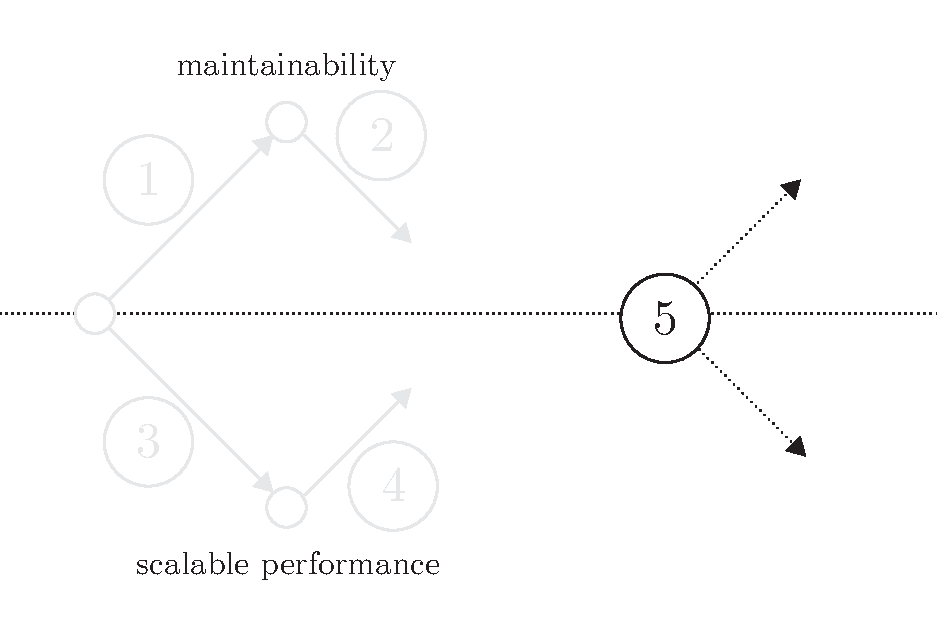
\includegraphics[width=0.6\textwidth]{../ressources/state-of-the-art-5.pdf}
\end{center}

The section \ref{chapter3:software-maintainability} shows that the modular organization enabled by functional programming is the best way to improve maintainability.
But it requires the use of a global memory store which conflicts with performance.
Compilation is a solution to reduce this conflict, but is not yet satisfactory enough for high performance scalability.
On the other hand, the section \ref{chapter3:software-performance} shows that to attain performance scalability, an application needs to multiply the exclusive accesses to its state.
That implies follow a distributed organization of its state to provide isolation and immutability, which negatively impacts modularity, hence maintainability.
Some works provide a uniform memory access to improve maintainability, despite the distributed execution.

The evolution of the economical constraints of a web application requires to repeatedly switch between maintainability and performance scalability.
The incompatibility between the two organizations implies technological ruptures at each switch.
Huge developing efforts are pulled to translate manually from one organization into the other, and later to maintain the implementation despites its unmaintainable nature.
There is still room for improvements on a compromise between maintainability and performance scalability.

The state of the art highlighted that
\begin{itemize}
\item maintainability requires lazy-evaluation and higher-order programming, section \ref{chapter3:software-maintainability:programming-models:functional-programming}, and
\item higher-order programming requires a global memory abstraction, section \ref{chapter3:software-maintainability:modular-programming:limitations},
\end{itemize}
Javascript is a functional language that features higher-order programming and a global memory abstraction.
% Moreover, its dynamic natures allows a lot of flexibility for the developers.
Moreover, node.js features a streaming approach with the event-loop execution model, similar to the lazy evaluation.
These reasons make Javascript a language of choice for developing web application.

And that
\begin{itemize}
\item scalable performance requires parallelism, and
\item parallelism requires exclusive accesses on the state through isolation and immutability.
\end{itemize}
Eventually, web development is heading toward a streaming approach with pipeline processing.

\nt{TODO dependency schema of these highlights}

This thesis proposes an equivalence between the global memory and control flow on one hand, and memory isolation with message passing on the other hand.
It proposes this equivalence as a solution to conciliate the scalable performance and maintainability.
As explained below, the concurrency model of the event-loop execution model, and the parallel approach of the pipeline execution model are very similar.
The goal of this thesis is to allow to compile one execution model into the other, to allow developers to constantly keep two organization of their implementation, allowing them to focus on both maintainability and scalable performance.

\subsection{Equivalence}

The next paragraphs introduces this equivalence between the event-loop execution model and the pipeline execution model.
The equivalence addresses two \textit{levels}\nt{not the good word}, as illustrated in figure \ref{fig:chapter3:objectives:roadmap}, the control flow, and the memory isolation.

\begin{figure}[h!]
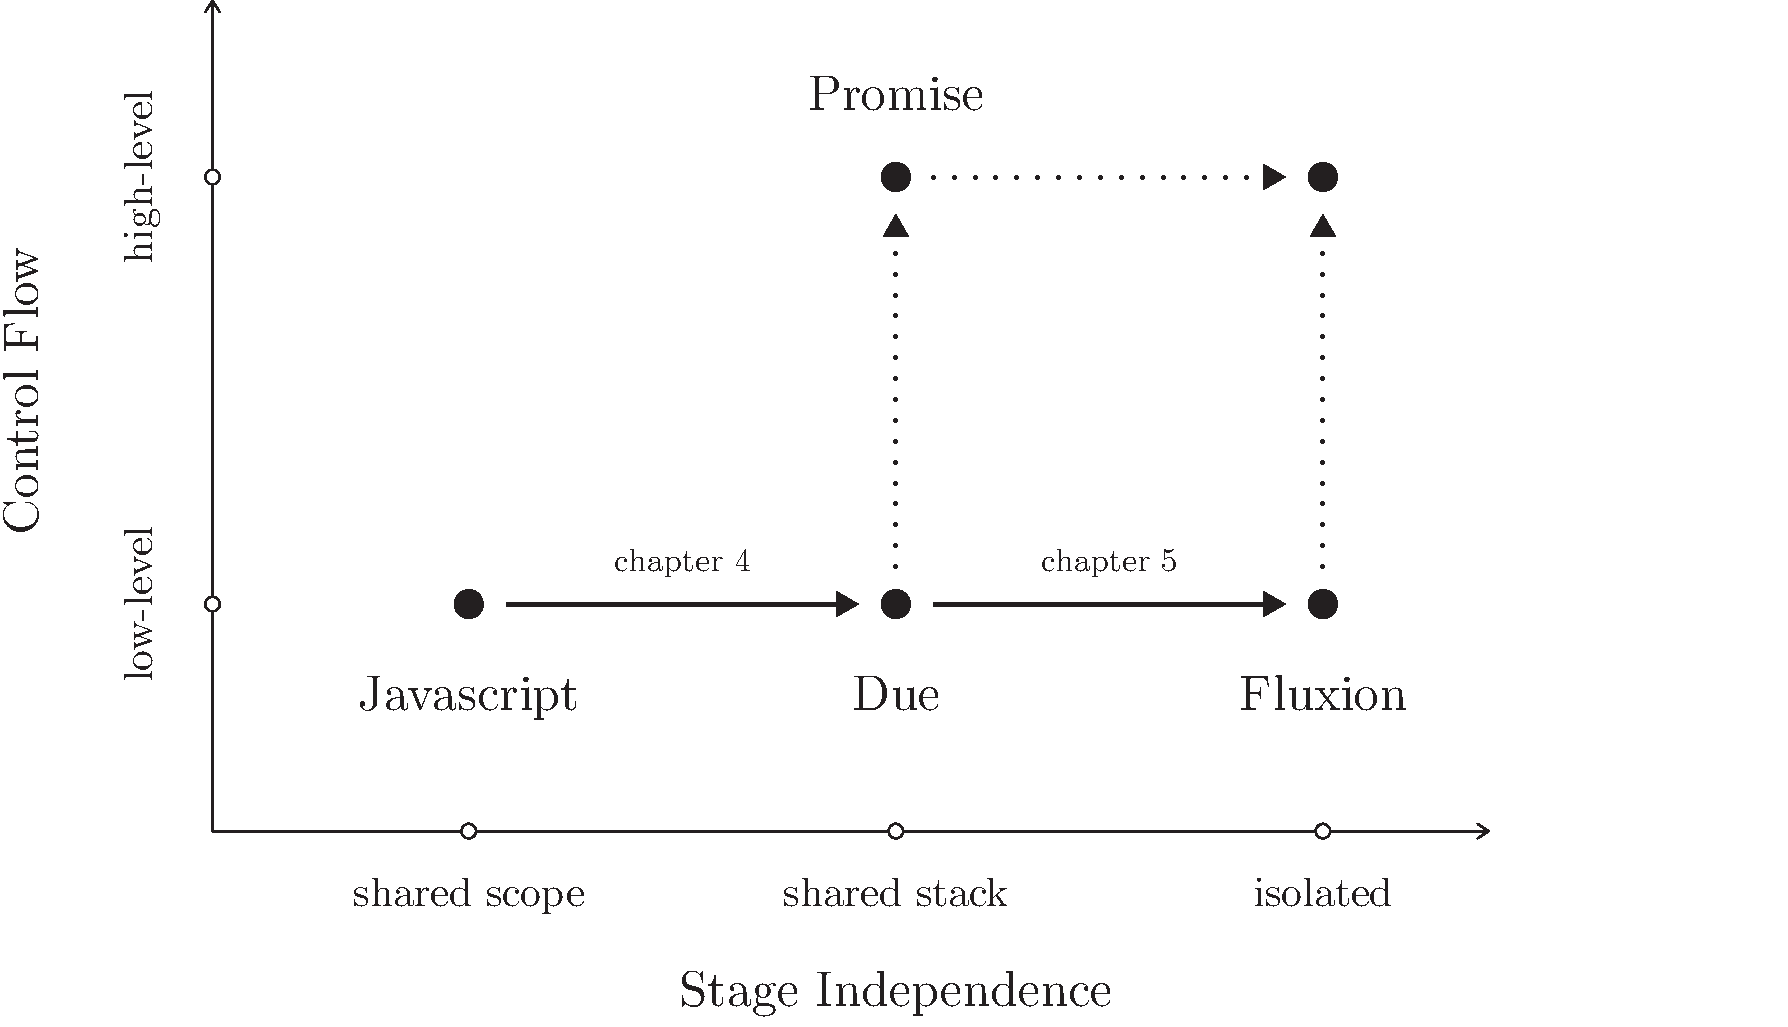
\includegraphics[width=1\textwidth]{../ressources/roadmap.pdf}
\caption{Roadmap}
\label{fig:chapter3:objectives:roadmap}
\end{figure}

\subsubsection{Rupture Point}

The execution of the pipeline architecture is well delimited in isolated stages.
Each stage has its own thread of execution, and is independent from the others.
On the contrary, the code of the event-loop is linear because of the continuation passing style and the common memory store.
% The message passing linking the callbacks is transparently handled by the event-loop.
However, the execution of the different callbacks are as distinct as the execution of the different stages of a pipeline.
The call stacks of two callbacks are distinct.
Therefore, an asynchronous function call represents the rupture between two call stacks.
It is a rupture point, and is equivalent to a data stream between two stages in the pipeline architecture.

Both the pipeline architecture and the event-loop present these rupture points.
The detection of rupture points allows to map a pipeline architecture onto the implementation following the event-loop model.
To allow the transformation from one to the other, this thesis studies the possibility to detect rupture points, and to distribute the global memory into the parts defined by these rupture points.
The detection of rupture points is addressed in chapter \ref{chapter4}.

It presents the extraction of a pipeline of operations from a Javascript application.
Indeed, such pipeline is similar to the one exposed by Promises.
The chapter proposes a simpler alternative to the latter called Dues.
However, these operations still require a global memory for coordination so they are not executed in parallel.

\subsubsection{Invariance}

% This transformation is important on two points.
% The conservation of the invariance.
% The equivalence between the coordinations.

The transformation should preserve the invariance as expressed by the developer to assure the correctness of the execution.
The partial ordering of events in a system, by opposition to total ordering, is sufficient to assure this correctness.
% This result was used by Lamport to prove the correctness of distributed systems.
The global memory is a way to assure the total ordering of events, and the message passing coordination is a way to assure partial ordering of events.
Therefore, to assure the correctness of the execution of a system, the state coordination with a global memory is equivalent to message passing coordination.
And it is possible, at least for some rupture points, to transform the global memory coordination into message passing while conserving the correctness of execution.

In order to preserve the invariance assured by the event-loop model after the transformation, each stage of the pipeline needs to have an exclusive access to memory.
The global memory needs not to be split into parts and distributed into each of the stages.
To assure the missing coordinations assured by the shared memory between the stages, the transformation should provide equivalent coordination with message passing.
The isolation and replacement of the global memory is fully address in chapter \ref{chapter5}, with the introduction of isolated containers called Fluxions.




% The invariance holds for the whole memory during the execution of each callback.
% As I explained in the previous section, this invariance is required to allow the concurrent execution of the different tasks.
% On the other hand, the invariance is explicit in the pipeline architecture, as all the stages have isolated memories.
% The coordination between these isolated process is made explicit by the developer through message passing.

% I argue that the state coordination between the callbacks requireing a global memory could be replaced by the message passing coordination used manually in the pipeline architecture.
% I argue that not all applications need concurrent access on the state, and therefore, need a shared memory.
% % Specifically, I argue that each state region remains roughly local to a stage during its modification.
% \nt{TODO review that, I don't know how to formulate these paragraphs. Identify the state and the data in the global memory.}

% \subsubsection{Transformation}

% This equivalence should allow the transformation of an event loop into several parallel processes communicating by messages.
% In this thesis, I study the static transformation of a program, but the equivalence should also hold for a dynamic transformation.
% I present the analyzis tools I developed to identify the state and the data from the global memory.



TODO Talk about the annotations used by many parallel languages.



Some links I NEED to put :
--------------------------

https://glyph.twistedmatrix.com/2014/02/unyielding.html
http://calculist.org/blog/2011/12/14/why-coroutines-wont-work-on-the-web/

Transitions :
  - Linkedin - http://engineering.linkedin.com/architecture/brief-history-scaling-linkedin
  - Facebook - https://www.cs.princeton.edu/events/event/evolution-software-architecture-facebook / http://www.infoq.com/presentations/Evolution-of-Code-Design-at-Facebook
  - ... 

https://medium.com/@benorama/the-evolution-of-software-architecture-bd6ea674c477

https://en.wikipedia.org/wiki/Dataflow
https://en.wikipedia.org/wiki/Real-time_computing
https://en.wikipedia.org/wiki/Partitioned_global_address_space
https://en.wikipedia.org/wiki/SPMD

Albert Cohen
https://scholar.google.com/citations?user=MkKZKAMAAAAJ&hl=en

+ Paul Feautrier (Tutor of A. Cohen)


SPMD Single program multiple data
Partitioned global address space


Similar problem :
http://2015.splashcon.org/event/splash2015-splash-i-lindsey-kuper-talk
http://www.cs.indiana.edu/~lkuper/papers/lindsey-kuper-dissertation.pdf

PJS was abandoned :
https://groups.google.com/forum/#!topic/mozilla.dev.tech.js-engine/H-YEsejE6DA
https://bugzilla.mozilla.org/show_bug.cgi?id=1117724

See parallel JS for further work (maybe) :
http://smallcultfollowing.com/babysteps/blog/2014/04/24/parallel-pipelines-for-js/

Some chunks I might find useful later :
---------------------------------------

\cit{No matter how great the talent or efforts, some things just take time. You can't produce a baby in one month by getting nine women pregnant.}
{Warren Buffett}

A good example of declarative sentence in everyday world : in case of fire, 
the elevators don't work -> you understand that you need to take the stairs.

The purpose of explicit synchronization is to manage the timing of side-effects in the presence of parallelism. 

A function is side-effect free if it is referentially transparent.



---


We presented in the introduction the popularity of Javascript, we argue that using this position to leverage parallelism is the only solution, and that proposing a new language, only on the base that it provide parallelism could not possibly make this language popular and grow a community.

Therefore, the only solution is to use the existing languages as is, and to compile them to gain parallelism.